\documentclass[12pt]{article}
\usepackage[english]{babel}
\usepackage{graphicx}
\usepackage[margin=3cm]{geometry}

\usepackage{amsmath, amssymb, amsthm}
\theoremstyle{plain}
\newtheorem{theorem}{Theorem}
\newtheorem{proposition}{Proposition}
\newtheorem{lemma}{Lemma}
\newtheorem{corollary}{Corollary}
\theoremstyle{remark}
\newtheorem*{remark}{Remark}
\newtheorem*{definition}{Definition}
\newtheorem*{exercise}{Exercise}
\newtheorem*{example}{Example}
\newtheorem*{warning}{Warning}

\newcommand{\boR}{\mathbb{R}}
\newcommand{\boC}{\mathbb{C}}
\newcommand{\boE}{\mathbb{E}}
\newcommand{\R}{\mathbb{R}}
\newcommand{\C}{\mathbb{C}}
\newcommand{\N}{\mathbb{N}}


\usepackage{listings}
\usepackage{hyperref}
\usepackage{courier}

%\usepackage{layout}
\usepackage{xcolor}
\definecolor{commentgreen}{RGB}{2,112,10}
\definecolor{eminence}{RGB}{108,48,130}
\definecolor{weborange}{RGB}{255,165,0}
\definecolor{frenchplum}{RGB}{129,20,83}
\definecolor{lgrey}{RGB}{235,235,235}

\newcommand{\cpp}{C\nolinebreak\hspace{-.05em}\raisebox{.4ex}{\tiny\bf +}\nolinebreak\hspace{-.10em}\raisebox{.4ex}{\tiny\bf +}}



\lstset{
  linewidth=17cm,
  %xleftmargin=0cm,
  %xrightmargin=-1cm,
}


\lstdefinestyle{C}{
  language=C,                     % choose the language of the code
  numbers=left,                   % where to put the line-numbers
  stepnumber=1,                   % the step between two line-numbers.        
  numbersep=10pt,                  % how far the line-numbers are from the code
  inputencoding=utf8,
  upquote=true,
  commentstyle=\color{commentgreen},
  keywordstyle=\color{eminence},
  stringstyle=\color{red},
  basicstyle=\footnotesize\ttfamily, % basic font setting
  emph={int,char,double,float,unsigned,void,bool,size_t,inline,template,auto,static},
  emphstyle={\color{blue}},
  showspaces=false,               % show spaces adding particular underscores
  showstringspaces=false,         % underline spaces within strings
  showtabs=false,                 % show tabs within strings adding particular underscores
  tabsize=8,                      % sets default tabsize to 2 spaces
  breaklines=false,                % sets automatic line breaking
  breakatwhitespace=true,         % sets if automatic breaks should only happen at whitespace
  title=\lstname,                 % show the filename of files included with \lstinputlisting;
  frame=tb,
  captionpos=tb,                  % sets the caption-position to bottom
  backgroundcolor=\color{lgrey},  % choose the background color. You must add \usepackage{color}
}

\lstdefinestyle{Python}{
  language=Python,                     % choose the language of the code
  numbers=left,                   % where to put the line-numbers
  stepnumber=1,                   % the step between two line-numbers.        
  numbersep=10pt,                  % how far the line-numbers are from the code
  inputencoding=utf8,
  upquote=true,
  commentstyle=\color{commentgreen},
  keywordstyle=\color{eminence},
  stringstyle=\color{red},
  basicstyle=\footnotesize\ttfamily, % basic font setting
  %emph={int,char,double,float,unsigned,void,bool},
  emphstyle={\color{blue}},
  showspaces=false,               % show spaces adding particular underscores
  showstringspaces=false,         % underline spaces within strings
  showtabs=false,                 % show tabs within strings adding particular underscores
  tabsize=4,                      % sets default tabsize to 2 spaces
  breaklines=false,                % sets automatic line breaking
  breakatwhitespace=true,         % sets if automatic breaks should only happen at whitespace
  title=\lstname,                 % show the filename of files included with \lstinputlisting;
  frame=tb,
  captionpos=tb,                  % sets the caption-position to bottom
  backgroundcolor=\color{lgrey},  % choose the background color. You must add \usepackage{color}
}

\lstdefinestyle{bash}{
	backgroundcolor=\color{lgrey},
	basicstyle=\color{black}\footnotesize\ttfamily\selectfont,
	breakatwhitespace=false,  
	breaklines=true,
	captionpos=b,
	commentstyle=\color{commentgreen},
	escapeinside={\%*}{*)},
	extendedchars=true,
	frame=none,
	keepspaces=true,
	keywordstyle=\color{green},
	%language=bash,
	morekeywords={@},
	numbers=none,
	showspaces=false,
	showstringspaces=false,
	showtabs=false,
	stepnumber=2,
	stringstyle=\color{weborange},
	tabsize=2
}

\usepackage{algorithm, algpseudocode, float}



\title{MU4MA016\\Algorithms and Data Structures\\for Computer Programming}
\author{Didier Smets}
\date{}

\begin{document}

\maketitle

\noindent 
{\bf Last updated :} Sep. 22th 2024

\medskip

\noindent
{\bf Schedule 2024 :}\\
Week 1 (Sep. 5th)  : Sec. 1\\
Week 2 (Sep. 12th) : Sec. 2.1 and part of 2.2\\
Week 3 (Sep. 19th) : End of Sec. 2.2 and Sec. 3.1\\
Week 4 (Sep. 26th) : 

\tableofcontents

\pagebreak

%%%%%%%%%%%%%%%%%%%%%%%%%%%%%%%%%%%%%%%%%%%%%%%%%%%%%%%%%%%%%%%%%%%%%%%%%%%%%%%
%%%%%%%%%%%%%%%%%%%%%%%%%%%%%%%%%%%%%%%%%%%%%%%%%%%%%%%%%%%%%%%%%%%%%%%%%%%%%%%
\section{Introduction}
%%%%%%%%%%%%%%%%%%%%%%%%%%%%%%%%%%%%%%%%%%%%%%%%%%%%%%%%%%%%%%%%%%%%%%%%%%%%%%%
%%%%%%%%%%%%%%%%%%%%%%%%%%%%%%%%%%%%%%%%%%%%%%%%%%%%%%%%%%%%%%%%%%%%%%%%%%%%%%%

The course being entitled {\bf Algorithms} and {\bf Data Structures} for {\bf
Computer programming}, in this introductory lecture we will briefly discuss each 
of these three words, trying to highlight by some simple examples the kind of
questions which will interest us in the following.

%%%%%%%%%%%%%%%%%%%%%%%%%%%%%%%%%%%%%%%%%%%%%%%%%%%%%%%%%%%%%%%%%%%%%%%%%%%%%%%
\subsection{Algorithm}
%%%%%%%%%%%%%%%%%%%%%%%%%%%%%%%%%%%%%%%%%%%%%%%%%%%%%%%%%%%%%%%%%%%%%%%%%%%%%%%

The following algorithm was originally described by Euclid in order to find
the greatest common divisor (gcd) between two positive integers $a$ and $b$.

\begin{algorithm}[H]
\caption{Euclid's algorithm (original version)}
\begin{algorithmic}
\Require $a, b$ are positive integers
\Function{gcd}{$a$, $b$}
\While{$a \neq b$}
\If{$a > b$}
\State $a \gets a - b$
\Else{}
\State $b \gets b - a$
\EndIf
\EndWhile
\State \Return a
\EndFunction
\end{algorithmic}
\end{algorithm}

The above description is called {\tt pseudo code}. It is intended to be read my
humans, and it must be unambiguous for humans. Instead, computer programs which
we will tackle later, are intended to be read by computers (compilers or
interpreters), which implies further restrictions on them (both syntaxic and
in terms of the operations available). 

Among the properties of algorithms, we will be particularly interested in the
following :
\begin{itemize}
\item Correctness : that is the least one should ask for, but it needs not be overlooked !
\item Complexity : both time and space complexity (to be explained below).
\item Ease of implementation : because in the end it will need to be turned
into a program.
\end{itemize}

\subsubsection*{Correctness}
In the case of Euclid's algorithm we could argue along
the following lines :
\begin{enumerate}
\item After each step of the while loop, $a$ and $b$ remain both
	positive\footnote{Note to french speaking students : in mathematical english
		{\bf positive} means ``strictement positif''; the french ``positif''
		is instead translated as {\bf non negative}.}
Indeed they must be different to enter the loop and the smaller is subtracted
from the larger. 
\item Because of the previous claim, the sum $a + b$ decreases strictly after
each step of the loop. In particular, there can be at most finitely many steps
of the loop and therefore the algorithm will always terminate.
\item Let $c$ be the actual greatest common divisor of $a$ and $b$. Then after
each step of the loop, $c$ is still a divisor of $a$ and $b$. Indeed, if a
number divides two other numbers, then it also divides their difference. Since
the algorithm eventually returns (the modified version of) $a$, let's call it
$d$, it follows that $c$ divides $d$.
\item We next claim that $d$ divides (the original values of) $a$ and $b$. To
prove this we argue as above, but backward. First, at the end of the while loop
we have $a = b = d$, and therefore $d$ divides both $a$ and $b$. Now if $d$
divides $a$ and $b$ after some (arbitrary) step of the loop, it also did at the
previous one. This is because if a number divides two other numbers, it also
divides their sum (and running a step backward correspond to changing one of
them to the sum of the two). 
\item In summary, we have shown on one hand that $c$ divides $d$ (in particular
$c \leq d$), and on the other hand that $d$ divides $a$
and $b$. By definition of $c$ being the greatest common divisor of $a$ and $b$,
it follows that $c = d$, which proves the correctness.
\end{enumerate} 

In many cases, proving algorithm correctness proceeds by showing that some form
of invariant is preserved during the process (especially when some loops are
involved). In the example above, the invariant was the divisibility by $c$.

\subsubsection*{Complexity}

As mentioned already, for all the algorithms we will study, we shall discuss both {\bf
time complexity} and {\bf space complexity}. These notions only make rigorous 
sense within a so-called {\it computation} and a {\it memory} model, but in short :
\begin{itemize}
\item The time complexity measures how much computations the algorithm
needs to perform in order to provide its result. Since the number may
depend on the input values, it is often useful to distinguish between
the worst case scenario and some form of average case.
\item The space complexity measures the amount of local storage required by
the algorithm in order to perform its computations, in addition to the storage
of its inputs.
\end{itemize}

In practice the two notions often pull in opposite directions, and the optimum 
is a matter of compromise.

\medskip

In the case of Euclid's algorithm, space complexity is trivial: no temporaries
are required since only updates of the original variables occur. Time complexity
(assuming that comparison and arithmetic operations can all be performed in
$O(1)$ time\footnote{As reasonable as it may look, in practice most
implementations would implicitly require that the input integers fit in some range
allowing them to be represented easily on the architecture, e.g. over 64bits, 
which by nature kills the whole meaning of $O()$ analysis, but that is what it
is...}) can easily be computed to be $O(\max(a, b))$, where the worst case
happens when one of the two values, say $b$, is $1$ (just think of the routing of the algorithm
in that case, leading to $a$ being decreased by $1$ at each step until it
reaches $1$). 

\medskip

The following variant is actually often called the Euclid algorithm too, 
although it was not presented by Euclid in this form.

\begin{algorithm}[H]
\caption{Euclid's algorithm (improved version)}
\begin{algorithmic}
\Require $a, b$ are positive integers
\Require $c$ a temporary storage for an integer
\Function{gcd}{$a$, $b$}
\While{$b \neq 0$}
\State $c \gets b$ 
\State $b \gets a \textrm{ modulo } b$
\State $a \gets c$
\EndWhile
\State \Return a
\EndFunction
\end{algorithmic}
\end{algorithm}

\noindent {\bf Exercise :} 
\begin{itemize}
\item Prove the correctness of this second version.
\item Prove that its time complexity is $O(\log(\max(a, b)))$.\\{\it Hint:
	proceed backward and compare the current values of $a$ and $b$ to the
		Fibonacci sequence defined by $F_0=0$, $F_1=1$ and $F_{k+2} =
		F_{k+1} + F_{k}$.}
\end{itemize}

In practical applications, a logarithmic complexity is a really strong 
and desirable one, in comparison e.g. here to the linear complexity of 
the original version. Even worse would be a quadratic, cubic, general polynomial
or even non polynomial (abbr. as NP) complexity.

%%%%%%%%%%%%%%%%%%%%%%%%%%%%%%%%%%%%%%%%%%%%%%%%%%%%%%%%%%%%%%%%%%%%%%%%%%%%%%%
\subsection{Data Structure}
%%%%%%%%%%%%%%%%%%%%%%%%%%%%%%%%%%%%%%%%%%%%%%%%%%%%%%%%%%%%%%%%%%%%%%%%%%%%%%%

Consider the following two variants of the birthday-matching problem (i.e.
determine if at least two among a class of students have the same anniversary
date, omitting year).

\begin{algorithm}[H]
\caption{Birthday match using sets}
\begin{algorithmic}
\Require As input, a set of students, called $class$
\Require As temporary storage, a set of students called $visited$
\State Initialize $visited$ as the empty set
\ForAll{student $a$ in $class$}
\ForAll{student $b$ in $visited$}
\If{$birthday\_match(a, b)$}
\State \Return true
\EndIf
\EndFor
\State Insert $a$ into $visited$
\EndFor
\State \Return false
\end{algorithmic}
\end{algorithm}

We have implicitly assumed here that we have a notion of {\it Set}, over which we can
{\it Iterate}, and which we can grow by making use of some {\it Insert}.

\medskip

An {\bf Abstract Data Structure (ADS)} is an abstract description of 
\begin{enumerate}
\item What kind of data can be stored (possibly referring to other existing ADS)
\item What operations can be performed on these data
\end{enumerate}


In terms of time complexity, in worst case scenarios we will need to apply
$O(N^2)$ (where $N$ is the number of students in class) times the birthday match
check. We should also take into account the time complexity associated to the
{\it Iterate} (for all) and {\it Insert} functions. These later must either be
postulated (as we did for the arithmetic operations in Euclid's), or guaranteed 
by some implementation of a Concrete Data Structure within a computing and
memory model.

\medskip

In terms of space complexity, the set $visited$ may grow at most to a size of
$N$. With the same caution as above regarding theory vs implementation, we will say that 
the space complexity is therefore $O(N)$.


Note that whenever $N > 365$, the algorithm could exit early with {\it true}, by
an immediate application of the pigeon-hole principle\footnote{If there are more pigeons than
cages, at least two pigeons must share the same cage. In french: ``Principe des
tiroirs''.} Not only this underlines
the caution that should always accompany asymptotic analysis in finite
frameworks, but it also suggests a very different variant~: 

\begin{algorithm}[H]
\caption{Birthday match using an array}
\begin{algorithmic}
\Require As input, a set of students, called $class$
\Require As temporary storage, an array $A$ of 365 boolean
\State Initialize all entries of $A$ with false
\ForAll{student $s$ in $class$}
\State Let $k$ be the anniversary date of $s$ (view as an integer $1 \leq k \leq 365$)
\If{$A[k] = true$}
\State \Return true
\Else
\State $A[k] \gets true$
\EndIf
\EndFor
\State Return false
\end{algorithmic}
\end{algorithm}

The time complexity of this variant is now only $O(N)$ (with the same caution as
before), and the space complexity is fixed, independently of the size of the
class, therefore $O(1)$.

\medskip

\noindent{\bf Exercise : } Replace 365 by an integer $M$ (imagine we compare
some ID numbers instead of birthdays), and assume that both $M$ and $N$ get
large but also that $M \gg N$ (by this we mean that $M$ is much larger than $N$)
and that a spatial complexity of $O(M)$ is forbidden because it would be too
large in practice. Are we forced to resort to the first version of the
algorithm, or could we do better ? ({\it Hint: hash tables and sorted trees are both in the
menu for later}).

\bigskip

The data structures that we shall go over in this course include : arrays,
stacks, queues, lists, hash tables, (binary search) trees, heaps and graphs.
Different implementations may use different concrete data structures to 
represent the same abstract data structure. The abstract notion of Set or of
Dictionary, is often implemented either via a hash table, or with some form
of tree. 

%%%%%%%%%%%%%%%%%%%%%%%%%%%%%%%%%%%%%%%%%%%%%%%%%%%%%%%%%%%%%%%%%%%%%%%%%%%%%%%
\subsection{Computer Programming}
%%%%%%%%%%%%%%%%%%%%%%%%%%%%%%%%%%%%%%%%%%%%%%%%%%%%%%%%%%%%%%%%%%%%%%%%%%%%%%%

We are not going to study computer programming per se\footnote{In particular this 
is not a course on the latest hype in \cpp !}, but we are going to study how to 
efficiently implement (good) algorithms on computers, using specific languages.

As scientific programmers, there are essentially two choices, which differ by 
their strong points and limitations.
\begin{itemize}
\item Using a high level language, offering a number of high level native data
structures, and potentially also an interactive interpreter. This is the case
e.g. of Python and its CPython interpreter, or of Julia with its 
just-in-time (JIT) compiler. This is the easiest to start with, 
and it can be efficient too when appropriate libraries (coded in low level
languages) are available for the task of choice, like e.g. Numpy just to name
one. This is also a very good test bed for profiling a new algorithm on small
data sets, before turning to a lower level language for performance on large 
scale data sets.
\item Using a lower level language, giving a closer access to the hardware or
at least to the virtual memory, and which can be compiled into efficient machine
code due to compiler optimizations. This is the case e.g. of C/\cpp, and the
one we will use in this course.
\end{itemize}

The syntax and grammar of C will not be taught in class. There are very good
references online, C grammar is easy, and those who have never met with it 
will catch-up quickly in the first TP classes. From \cpp (kind of a superset of
C) we will only ever borrow a few features that {\it may} sometimes be handy.

\medskip

Although lower level languages are said to be closer to the hardware, in
this course for the most we will only need to understand an take into
account the following. The storage memory is presented to us by the 
operating system (OS) as a large addressable 1D array, the so-called 
{\it virtual memory}, and
\begin{enumerate}
\item 
{\bf The access time needed to bring back some data from RAM to the CPU can
be much larger than the typical time needed by the CPU to perform some
		computation/instruction} (one
usually measures time in so-called CPU cycles). As of today, it can be by a 
factor 100x to 1000x, with respect e.g. to an arithmetic operation.
\item
In order to overcome this otherwise huge bottle-neck in computation, a number of 
physical levels of so-called caches are introduced in between the CPU and the RAM. 
You can think of these cache levels as smaller but faster access memories, and
there are strategies (independent of us) to decide what is kept in cache (I
like the analogy of RAM being the university library, the next level of cache 
is your home bookshelf, and the closest level of cache to CPU is your
nightstand). {\bf The
important thing to remember as a programmer, is that if some data is put into cache,  
then the ``nearby'' data (in the virtual memory 1D array) is brought at the same time, 
and therefore it will be readily available provided our successive accesses to memory 
are sufficiently local}. 
\end{enumerate}

This notion of {\it locality} is well understood (and can be experienced!) in the following
simple yet typical example of the computation of the product $A * B$ of two
matrices, say of size $N \times N.$

\medskip

Let's first implement it (in language C) in the way you were taught about the matrix
product in Math classes. Note first that the memory being a 1D array, matrices need to
be ``flattened'' to be recorded in memory. The so-called {\it row-major} convention, 
i.e. line after line, where the equivalent of what we write $A(i,j)$ in math is
accessed in $A[i * N + j]$, is the most popular in C language implementations. 
The other obvious alternative, the so-called {\it column-major} convention, was 
most popular in Fortran language. Which algorithm works best for a matrix
product is highly dependent of the choice of the convention, as we shall
experience ! In the sequel we choose the {\it row-major} standard C
convention. Note also that in C, indices for array indexing start at $zero$,
not at $1$ as we usually do in math, this eases address computations.  

\begin{lstlisting}[style=C]
void matrix_product1(float C[], const float A[], const float B[], int N)
{
	for (int i = 0; i < N; ++i) {
		for (int j = 0; j < N; j++) {
			/* Compute C_{i,j} */
			C[i * N + j] = 0;
			for (int k = 0; k < N; k++) {
				C[i * N + j] += A[i * N + k] * B[k * N + j];
			}
		}
	}	
}
\end{lstlisting}

When the loop counters $i$, $j$ or $k$ are incremented, the data locations involved in the
actual product computation on line 8 vary differently. An increment of $i$ leads
to a jump of $N$ (times the size of a float, not repeated later) in memory for $C$ and $A$. An
increment of $k$ introduces a jump of $N$ in the memory location for $B$, and finally an
increment of $j$ only induces increments of one (i.e. no jump, i.e. local). 
By far the most problematic of all these is the jump of $N$ introduced by an
increment of $k$ : indeed it arises at every of the $N^3$ steps of the three
nested loops. The increment of $i$ causes the same jump of $N$, but it only
occurs $N$ out of the $N^3$ steps, which is negligible in proportion. This
implementation, at least for large values of $N$, will therefore likely 
be memory bottlenecked.

\medskip

Instead, let us propose the following alternative obtained for the most 
by a permutation of the loops in $j$ and $k$ :
\begin{lstlisting}[style=C]
void matrix_product2(float C[], const float A[], const float B[], int N)
{
	for (int i = 0; i < N; ++i) {
		/* Zero initialize C */
		for (int j = 0; j < N; j++) {
			C[i * N + j] = 0;
		}
		for (int k = 0; k < N; k++) {
			for (int j = 0; j < N; j++) {
				/* Update C_{i,j} */
				C[i * N + j] += A[i * N + k] * B[k * N + j];
			}
		}
	}	
}
\end{lstlisting}

\noindent{\bf Exercise :} First convince yourself that this second version also
actually computes the product of $A$ and $B$ ! Then analyze the memory accesses
as above, and observe that the non local jumps only occur now $N^2$ out of $N^3$
times, which is negligible in proportion if $N$ is large, and therefore should 
better avoid the memory latency problem.

\medskip

\noindent{\bf Exercise :} Check it in practice by testing e.g. with $N = 1000$, 
after you will be familiar with C and gcc in the first TP classes. 
In these tests, try both the compiler optimization {\tt -O0} (i.e. no
optimization) and {\tt -O3} (most optimizations).

\medskip

\noindent{\bf Proposed solution}
Here is a proposed test implementation, that will serve for those of you
discovering C. Reproduce and test on your own !

\lstinputlisting[style=C]{data/matrix_multiplication_test.c}

We then compile it (first with zero optimization) :

\begin{lstlisting}[style=bash]
@: gcc -Wall matrix_multiplication_test.c -o matrix_multiplication_test
\end{lstlisting}

and test it

\begin{lstlisting}[style=bash]
@: ./matrix_multiplication_test 1000
Timer Algo 1: 4.159 s
Sum of C : 250005104.000000
Timer Algo 2: 3.229 s
Sum of C : 250005104.000000
\end{lstlisting}

We can observe a modest difference but not great. Let's introduce compiler
optimization (level 3 = all).

\begin{lstlisting}[style=bash]
@: gcc -Wall -O3 matrix_multiplication_test.c -o matrix_multiplication_test
@: ./matrix_multiplication_test 1000
Timer Algo 1: 1.031 s
Sum of C : 250005104.000000
Timer Algo 2: 141.192 ms
Sum of C : 250005104.000000
\end{lstlisting}

First as you can see the -O3 flag implied a great speed-up, but more importantly 
the {\tt\_v2} version of the algorithm also now runs one order of magnitude faster than 
the {\tt\_v1} one !

\medskip

\begin{remark} Although the matrices $A$ and $B$ 
were filled with random real numbers between 0 and 1, the sum of 
the coefficients of $C$ seems to be an integer. How is that possible ?!\\ 
The (pseudo)-random values stored in $A_{ij}$ and $B_{jk}$  are supposed
to model a uniform distribution on $[0,1]$, therefore
$$
\boE(sum(C)) = \sum_{i,j,k = 1}^N \boE(A_{ij}B_{jk}) =  \sum_{i,j,k = 1}^N
\boE(A_{ij}) \boE(B_{jk}) = \frac{N^3}{4},
$$
where we have used that $A_{ij}$ and $B_{jk}$ are independent (they are
different samplings of the random variable) and $\boE(A_{ij}) = \boE(B_{jk}) =
\frac{1}{2}$ for a uniform variable over $[0,1]$. For $N = 1000$, we expect therefore
that $\boE(sum(C)) = 2.5e8$, which indeed is an integer. But the error itself,
in the example sampling above $5104$, has no reason to be an integer. This is
not at all related to the maths, but instead to the way real numbers (here 32
bits floating points) are stored in a computer, we will discuss that into more
details later. 
Not all real numbers are represented (there would be infinitely
many of them!), and it happens that within 32bits floats the closest float to
$2.5e8$ is $2.5e8 + 1.$ If you take $N = 100$ instead, you'll start
observing fractional parts in the answer.
\end{remark}

\noindent
{\bf Exercise :} Compute that
$$
\boE(sum(C)^2) = \frac{1}{16}N^6 + \frac{1}{24}N^4 + \frac{1}{36}N^3
$$
and therefore that 
$$
\Sigma(sum(C)) = \sqrt{Var(sum(C))} = \sqrt{N^4/24 + N^3/3} \simeq 0.2 N^2
\text{ for N large}.
$$
Run the test above multiple times, of with different values of $N$, and
observe/check then that the deviation to the expected value is indeed 
of the order of the standard deviation $\Sigma(sum(C)) \simeq 0.2 N^2$.\\
{\it Hint : while evaluating terms of the form
$\boE(A_{ij}B_{jk}A_{i'j'}B_{j'k'})$, distinguish between the three cases : 
a) $(i,j,k) = (i',j',k')$, b) $(i,j) = (i',j')$ or $(j,k)=(j',k')$ but $(i,j,k)
\neq (i',j',k')$, and finally c) $(i,j) \neq (i',j')$ and $(j,k) \neq (j',k')$. 
Recall also that whenever $X$ is uniform over $[0,1]$, $\boE(X^2) = 
\int_0^1 x^2\, dx = \frac{1}{3}$.} 

\medskip

Finally, let us compare our code performance with respect to Python, either
using pure Python loops or using available scientific libraries, the most
famous being Numpy (it is internally coded in C!).

\lstinputlisting[style=Python]{data/matrix_multiplication_test.py}

We obtain :  

\begin{lstlisting}[style=bash]
@: python3 matrix_multiplication_test.py
Pure Python for N =   10 : 0.00117s
Pure Python for N =   20 : 0.00923s
Pure Python for N =   50 : 0.07167s
Pure Python for N =  100 : 0.52314s
Pure Python for N =  200 : 4.19137s
Using Numpy for N = 1000 : 0.00737s
Using Numpy for N = 2000 : 0.04697s
Using Numpy for N = 4000 : 0.35011s
\end{lstlisting}

A number of remarks are in order :
\begin{enumerate}
\item
For both algorithm, we can observe the expected behaviour of a cubic time
complexity. Note that algorithm with a lower power of $N$ do exist (see e.g. 
this \href{https://en.wikipedia.org/wiki/Computational_complexity_of_matrix_multiplication}{Wiki link}),
but they are complex to implement and often come with large pre-factor
constants. The most well-known is Strassen's algorithm, at $O(N^{\log_2(7)})
\simeq O(N^{2.8})$, but the present state of the art is $O(N^{2.37})$. Clearly 
any algorithm must be at least $O(N^2)$ (indeed at least the $N^2$ entries of
$C$ must be filled!), at least for a sequential algorithm, but it is open if 
one could go as low as $O(N^2)$.
\item
There is a {\bf huge} difference between the timings in pure Python and using
Numpy, more than three orders of magnitude. As a matter of fact, for pure Python I 
had to limit $N$ to a smaller value than a few hundreds in order to keep the script run 
time under control.
\item 
For $N = 1000$, Numpy is still 20 times faster that our current best
implementation in \tt{\_v2} !
\end{enumerate}

What can/should we do to improve our code to state of the art performance then ?

There are easy improvements :
\begin{enumerate}
\item Allow the compiler to use the whole set of CPU instructions for the computer
we are running on (this can be an issue if we wish to distribute our program to
machines which would not have all this set). The gcc option is {\tt -march =
native}. A safer yet usually as effective solution is to require a common vector
instruction set, like the MMX or AVX. We shall use the {\tt -mavx} gcc switch.
\item Modify our C code by adding the {\it restrict} keyword to the output array
pointer C of our matrix\_product functions. This tells the compiler that the place where
we write $C$ does not overlap (one says ``aliases with'') the one of $A$ and or
$B$, and avoids unnecessary copies. 
\item Modify our C code by forcing a 256 bits alignment for our
memory allocations of $A, B$ and $C$. This can improve the use of vector
instructions by the compiler (see 1) here above). To do so, we replace 
{\tt malloc} by {\tt aligned\_alloc}.
\end{enumerate}

\begin{lstlisting}[style=C]
void matrix_product_v2(float *__restrict C, const float *A, 
						const float *B, int N) {
[...]
}

[...]
	float *A = (float *)aligned_malloc(32, N * N * sizeof(float));
	float *B = (float *)aligned_malloc(32, N * N * sizeof(float));
	float *C = (float *)aligned_malloc(32, N * N * sizeof(float));
[...]
\end{lstlisting}
With these and the avx switch we obtain:
\begin{lstlisting}[style=bash]
@: gcc -Wall -O3 -mavx matrix_multiplication_test.c -o matrix_multiplication_test
@: ./matrix_multiplication_test 1000
Timer Algo 1: 1.042 s
Sum of C : 250279296.000000
Timer Algo 2: 69.523 ms
Sum of C : 250279296.000000
\end{lstlisting}
We have improved from $140ms$ to $70ms$, that is a factor 2, not bad ! Be we
are still missing a factor almost 10. Let us observe the Operating System 
Monitor, first during our own implementation : 
\begin{center}
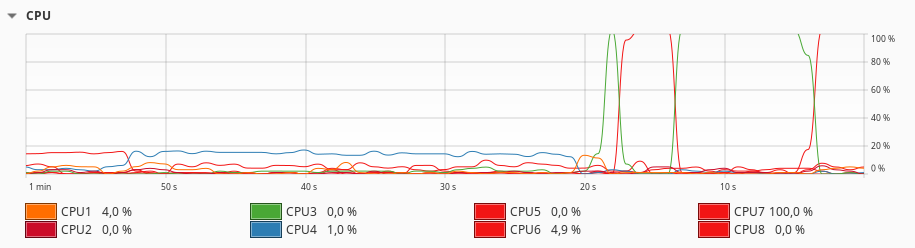
\includegraphics[width=15cm]{data/mat_mult_one_core.png}
\end{center}
and then during Numpy's implementation\footnote{In both cases, we have increased
$N$ so has to have time to take a screenshot !} 
\begin{center}
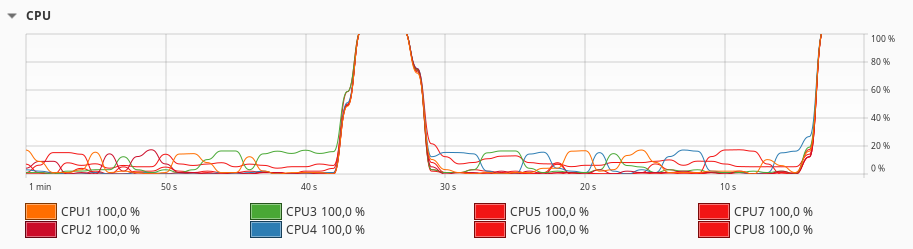
\includegraphics[width=15cm]{data/mat_mult_all_core.png}
\end{center}

The road-map is clear : our code is sequential, it uses just one CPU core, while
Numpy is making use of parallelism to use all the available 4 cores / 8 threads
in my (modest) computer ! 

\medskip

Numpy's (quite complex) source code can be browsed on Github 
\href{https://github.com/numpy/numpy/tree/main}{here}. One C source
file for (one of the possible versions of) matrix multiplication is
\href{https://github.com/numpy/numpy/blob/main/numpy/_core/src/umath/matmul.c.src}{this
one}. It has many includes and internal preprocessor macros making it difficult 
to read though, you may even have difficulties to recognize a valid C code.   

\medskip

Turning our matrix multiplication code into a parallel algorithm is one of the
very nice projects that you could implement for this course, especially for
those of you that are in the HPC program. Either making use of
CPU parallelism (using e.g. {\tt OpenMP} or better the lower level {\tt
pthread}), or even going to the GPU if one is 
available on your computer (using e.g. {\tt OpenCL}, {\tt OpenGL/Vulkan} 
compute shaders, or the proprietary {\tt CUDA}).

\medskip

In a broader perspective, parallelization of algorithms in many different areas
of Math/CS has been a very hot topic in recent years. This yields challenges both at the
algorithmic level, and at the implementation level. They require specific courses 
and we shall not dive too deeply into it, yet they all build upon the concepts
we shall develop in this course.


%%%%%%%%%%%%%%%%%%%%%%%%%%%%%%%%%%%%%%%%%%%%%%%%%%%%%%%%%%%%%%%%%%%%%%%%%%%%%%%
%%%%%%%%%%%%%%%%%%%%%%%%%%%%%%%%%%%%%%%%%%%%%%%%%%%%%%%%%%%%%%%%%%%%%%%%%%%%%%%
\pagebreak
\section{Some programming concepts}
%%%%%%%%%%%%%%%%%%%%%%%%%%%%%%%%%%%%%%%%%%%%%%%%%%%%%%%%%%%%%%%%%%%%%%%%%%%%%%%
%%%%%%%%%%%%%%%%%%%%%%%%%%%%%%%%%%%%%%%%%%%%%%%%%%%%%%%%%%%%%%%%%%%%%%%%%%%%%%%

%%%%%%%%%%%%%%%%%%%%%%%%%%%%%%%%%%%%%%%%%%%%%%%%%%%%%%%%%%%%%%%%%%%%%%%%%%%%%%%
\subsection{Interface vs Implementation}
%%%%%%%%%%%%%%%%%%%%%%%%%%%%%%%%%%%%%%%%%%%%%%%%%%%%%%%%%%%%%%%%%%%%%%%%%%%%%%%

It is always useful and also often important to separate what we will call the 
{\it interface} from what we will call the {\it implementation}. In the table
below I have listed a number of concepts : all the ones in the left column
correspond (and may be more or less understood as equivalent between each
other) to the interface, while all the ones in the right column correspond to
the implementation.

\medskip

\begin{center}
	\begin{minipage}[t]{0.45\textwidth}
	On the user side :
	\begin{itemize}
		\item Abstract Data Structure
		\item Interface / Documentation
		\item Application Programming Interface (API)
		\item Header files\\
			In C/\cpp, typically {\tt .h} or {\tt .hpp}
	\end{itemize}
\end{minipage}
	\begin{minipage}[t]{0.45\textwidth}
	On the programmer side :
	\begin{itemize}
		\item Concrete Data Structure
		\item Implementation
		\item Source code\\\mbox{ }
		\item Source files\\In C/\cpp, typically {\tt .c} or {\tt .cpp}
	\end{itemize}
\end{minipage}
\end{center}

In vague terms the interface {\it should} : 
\begin{itemize}
	\item describe what kind of data it is designed to handle
	\item describe what actions on this data it can perform
	\item possibly offer some guarantee about algorithmic complexity of
		some of these actions (worst case, expected mean, etc).
\end{itemize}

It should {\it not} describe {\it how} these are implemented. One of the reasons
for the latter is the ability to update/improve the implementation without
breaking user code.

\medskip

A key point to have in mind when designing interfaces and implementations is
that less methods/actions available in the interface implies :
\begin{itemize}
	\item less flexibility for the user
	\item less constraints for the implementation, and therefore possibly
		better performance
\end{itemize}
As a rule of thumb : one should not devise overcomplicated data structures, but
choose the simplest one(s) that fit all the identified requirements for a task,
but no more. Some people call it the KISS philosophy : Keep It Straight and
Simple.

\medskip

An example in the standard C library which one encounters in the very first
steps of learning the language is the {\tt FILE} abstract data structure
for file IO (i.e. reading and writing to files).

Some typical code would look like

\begin{lstlisting}[style=C]
#include <stdio.h>

// [some code here]

FILE *f;  
f = fopen("example.txt", "r");
if (f == NULL) {
	// [produce error message and exit]
}

// [do something with f]

fclose(f);
\end{lstlisting}

What exactly is contained in {\tt FILE} needs not be known to us\footnote{It is actually
a macro for a (complicated) C struct defined in stdio.c}, we shall use it only as
a {\it opaque handle}. In the {\it header} file {\tt stdio.h} we can
find\footnote{On Linux systems this file is found in {\tt /usr/include/stdio.h}} 
(among other things) the {\bf declaration}~:
\begin{lstlisting}[style=C]
FILE *fopen(const char *__filename, const char *__modes);
\end{lstlisting}
which teaches us that the function {\tt fopen} :
\begin{itemize}
	\item requires two arguments, both of which being of type 
		{\tt char *} (used to represent character strings) and 
		which won't be modified by the function itself (because they 
		are marked with the keyword {\tt const}).
	\item returns a pointer to a {\tt FILE} data structure.
\end{itemize}
Most of the time, to access documentation for standard libraries you will
instead refer to online documents, like e.g. 
\url{https://cplusplus.com/reference/cstdio/fopen/} in the above case.

\medskip

Whenever we need to do something with the file, we must use the handle (it is
called {\tt f} is the sample code above) and pass it to the relevant function,
as in~:
\begin{lstlisting}[style=C]
// [do something with f]
char line[80];
fread(line, 80, f);
\end{lstlisting}

%%%%%%%%%%%%%%%%%%%%%%%%%%%%%%%%%%%%%%%%%%%%%%%%%%%%%%%%%%%%%%%%%%%%%%%%%%%%%%%
\subsection{Pointer based vs Array based implementation}
%%%%%%%%%%%%%%%%%%%%%%%%%%%%%%%%%%%%%%%%%%%%%%%%%%%%%%%%%%%%%%%%%%%%%%%%%%%%%%%

The implementation of data structures can usually be divided into two families : 
\begin{enumerate}
	\item Array based
	\item Pointer based
\end{enumerate}
The difference between both amounts to the way the data is stored in virtual
memory. 

\medskip

When array based, the data is stored in a {\it contiguous} way and it is
assumed that each element of the array occupies the same amount of space in
memory. The main implication of this is that to recover the element of index
{\tt k}, it suffices to fetch memory at the address being computed as the address
of the start of the array plus {\tt k} times the size of an array element. In
other words, only the address of the start of the array needs to be recorded. 

When pointer based instead, the data may be spread across memory. The implication is
that each element of the data should be accompanied with a way to access the
next and or the previous one(s), typically by storing its/their address(es).


\medskip
\noindent
We can therefore quickly foresee the advantages and limitations of both~: 
\begin{itemize}
	\item Array based are potentially much faster because they allow for
		direct access to any element by its index and need not store 
		addresses. On the other hand,
		the contiguity assumption has some implications on some
		operations (e.g. suppressing an element would imply a
		potentially large copy in order to avoid creating a gap, and the
		same would apply to some insertion in the middle). The
		question of how large the reserved memory chunk to store the
		array should be chose is also an important question, especially
		when it is not known a priori how large the data structure will
		be eventually (imagine we read elements from a file, and we only
		know we are finished when we reach its end).
	\item Pointer based have the exact opposite advantages and limitations. 
		Adding and/or suppressing elements is conceptually and
		practically simpler, because it only implies modifying a
		couple of pointers, but that may come at the price of
		performance. Besides, direct access to the k-th element 
		(whenever it makes sense, not all structures have a natural
		mapping to sequences, think e.g. of arbitrary trees) 
		is typically not possible for them.
\end{itemize}

To provide an example of both, and having the goal of separation 
interface/implementation in mind, in the sequel we propose one common 
interface and two possible implementations for a {\it Stack} data structure.
This is one of the simplest data structures, and it will therefore serve well
our expository purposes. The first implementation will be pointer based, while 
the second will be array based. 
User code should should equally work in both cases, as a matter of fact there
is nothing in the interface suggesting how it is implemented.

\medskip
\noindent
First the interface~:
\lstinputlisting[style=C]{data/stack.h}

\noindent
Next the pointer based implementation :
\lstinputlisting[style=C]{data/stack_pointer_based.c}

\noindent
And finally the array based one :
\lstinputlisting[style=C]{data/stack_array_based.c}

\noindent{\bf Exercise :} Assuming the cost of a memory allocation for a block
of size $M$ is $O(M)$, compute that using the doubling strategy for the array
capacity in the previous implementation, the average cost for $N$ successive
pushes to the stack is only $O(1)$. Instead, realize that any strategy which
would be based on a fixed additive capacity increase (rather than a 
multiplicative strategy) would lead to an $O(N)$ average cost. The factor 2 is
not important though, any (possibly non integer) number $r>1$ would accomplish
the same goal.  

%%%%%%%%%%%%%%%%%%%%%%%%%%%%%%%%%%%%%%%%%%%%%%%%%%%%%%%%%%%%%%%%%%%%%%%%%%%%%%%
\subsection{Inlining}
%%%%%%%%%%%%%%%%%%%%%%%%%%%%%%%%%%%%%%%%%%%%%%%%%%%%%%%%%%%%%%%%%%%%%%%%%%%%%%%

This subsection can be skipped at first reading, and is mostly meant for students 
that already have a compiled languages background.

In some cases, a clear separation between the interface and the implementation 
implies some performance costs which are undesirable. This situation arises
when some utility functions which are implemented are so small and used so often 
that the function calls themselves end-up accounting for most of the total cost.

\medskip

To avoid these situations, it is sometimes therefore advisable to {\it not}
separate both the interface and the implementation, so that the compilers will
always view the whole code of the given functions when including them elsewhere,
and will be able to optimize it better.

\medskip

As a typical example, the next listing proposes an implementation for an array
data structure. It is very much similar to the above array based implementation 
of a stack data structure, but promoted to an array data structure by adding 
random access to any index in the array. This is also the occasion to introduce some
\cpp that wouldn't compile as C code : it uses {\it templates}, and {\it methods} (in particular
constructors and destructors). Both concepts are not present (at least
as such) in plain C. They are mostly conveniences for the programmer, and 
they should be approached with care : do not over-abuse templates if you wish 
your code to compile fast, and pay attention to unnecessary copies in constructors 
it you wish your code to run fast !

\lstinputlisting[style=C]{data/array.hpp}

If you are familiar with \cpp, that may remind you of the {\tt std::vector} data
structure from the Standard Templated Library (STL). Pay attention though that
the {\tt TArray} version above is only really meant for types $T$ that are POD 
(Plain Old Data), i.e. types that can simply be bitwise copied and in particular 
have no need for constructors or destructors. In scientific computing the latter
are more important and more frequent for the ``real data''.



\pagebreak

We shall now discus the problem of {\bf Searching} in a data 
structure, i.e. looking for some data based on its {\it value}. 

\medskip

To make Searching efficient, data structures rely mostly on one or the other
of the following two key ideas :

\begin{itemize}
	\item Sorting
	\item Hashing
\end{itemize}

In Section \ref{sec:sort} we begin by discussing sorting, in the simple case 
of arrays, and how it improves searching by e.g. the binary search. 
In Section \ref{sec:hash} we will discuss hashing, and
the important related data structure the hash table. Further along we will go 
back to the question of sorting when discussing data structures which implement 
sorting while not not being (necessarily) arrays, like (self balancing) 
binary search trees in section \ref{subsec:bst} and \ref{subsec:sb}.


%%%%%%%%%%%%%%%%%%%%%%%%%%%%%%%%%%%%%%%%%%%%%%%%%%%%%%%%%%%%%%%%%%%%%%%%%%%%%%%
%%%%%%%%%%%%%%%%%%%%%%%%%%%%%%%%%%%%%%%%%%%%%%%%%%%%%%%%%%%%%%%%%%%%%%%%%%%%%%%
\section{Sorting}\label{sec:sort}
%%%%%%%%%%%%%%%%%%%%%%%%%%%%%%%%%%%%%%%%%%%%%%%%%%%%%%%%%%%%%%%%%%%%%%%%%%%%%%%
%%%%%%%%%%%%%%%%%%%%%%%%%%%%%%%%%%%%%%%%%%%%%%%%%%%%%%%%%%%%%%%%%%%%%%%%%%%%%%%

If an array of size $N$ isn't sorted, the average number of comparisons needed
when searching for some data in the array is clearly $O(N).$ 

If the array is known to be sorted (say in increasing order), we can improve the
search time complexity by relying on the following binary search strategy ({\it
recherche dichotomique} in french).

\begin{lstlisting}[style=C]
// @size : number of elements in the array
// @value : value which is searched for
float *binary_search(const float *array, size_t size, float value)
{
	size_t begin = 0;
	size_t end = size - 1;

	while (begin <= end) {
		size_t pos = (begin + end) / 2;
		if (array[pos] == value) {
			return (&array[pos]);
		} else if (array[pos] <= value) {
			begin = pos + 1;
		} else {
			end = pos - 1;
		}
	}
	/* If we reach here value is not present in the array */
	return NULL;
}
\end{lstlisting}

At each step in the while loop the length of the search interval is divided by
two (up to one due do integer division) until the value is found of the size of
the search interval drops down to nothing. In particular, their will be at most
$O(\log_2(N))$ such steps. 

Note that the float type could be replaced by an arbitrary type $T$ (like a user
defined struct) provided the latter implements and equality and comparison 
operators : 

\begin{lstlisting}[style=C]
// T should be an existing type, implementing 'is_equal' 
// and 'is_smaller'.
T *binary_search(const T *array, size_t size, T value)
{
	size_t begin = 0;
	size_t end = size - 1;

	while (begin <= end) {
		size_t pos = (begin + end) / 2;
		if (is_equal(array[pos], value)) {
			return (&array[pos]);
		} else if (is_smaller(array[pos], value)) {
			begin = pos;
		} else {
			end = pos;
		}
	}
	return NULL;
}
\end{lstlisting}

{\it Pay attention} that for the previous to work, the comparison function {\tt
is\_smaller} should implement an order and not just a pre-order on T. This remark
is important because in computer science it is common to use pre-orders. These
often have the form of an actual order, but acting only on part of the instances
of the given type
(typically a classical arithmetic compare on one distinct field of a struct -
think  e.g. of 2D points being ranked according to their x coordinates).
If the anti-symmetry property (that is a is smaller than b and b is smaller than
a implies that a is equal to b) is not satisfied, then the above algorithm may 
pick the wrong left or right side in such situations, and therefore would be
buggy. Most sorting algorithms are relevant and perfectly work in the case of 
pre-orders though, the reason why we mention it.


We will next discuss three sorting algorithms. They have been chosen because of
both their theoretical and practical importances.

%%%%%%%%%%%%%%%%%%%%%%%%%%%%%%%%%%%%%%%%%%%%%%%%%%%%%%%%%%%%%%%%%%%%%%%%%%%%%%%
\subsection{Insertion sort}
%%%%%%%%%%%%%%%%%%%%%%%%%%%%%%%%%%%%%%%%%%%%%%%%%%%%%%%%%%%%%%%%%%%%%%%%%%%%%%%

Insertion sort is one among if not the fastest sorting algorithm for small
arrays. It used also in best in class implementations for large arrays, but
in combination with other methods then (e.g. in the later merge sort when 
the array chunk size decreases below some predetermined value).  It is also
of theoretical value because it is one of the few cases where an average
time complexity can be rigorously derived without too much pain. At $O(N^2)$,
that complexity explains why it can be used alone for large values of $N.$

The algorithm can be described as follows : at iteration number $i$ the first
$i$ elements of the array have already been shuffled between themselves so 
that they are in order. The $i^{th} + 1$ element is then simply moved towards
the start of the array as long as it is in wrong order with respect to its
predecessor. The latter is achieved by a (possibly empty) sequence of swaps. 
The fact that the algorithm is in-place (which means that the array is sorted
directly with no need of a prior copy or equivalent, that is in $O(1)$ spatial 
complexity) and that it only uses swaps which by nature are memory cache
friendly, explains its speed for small inputs.

\begin{lstlisting}[style=C]
// Sort in increasing order 
void insertion_sort(float *A, int size)
{
	for (int i = 1; i < size; ++i) {
		int j = i;
		while (j > 0 && A[j] < A[j-1]) {
			float tmp = A[j];
			A[j] = A[j - 1];
			A[j - 1] = tmp;
			j--;
		}
	}
}
\end{lstlisting}

Before we compute the time complexity for a general input array, let us make the
following simple observation :
\begin{itemize}
	\item If the original array $A$ is already in order,
		then only one comparison (and no swap) will happen at each step
		of the outer loop. This makes yields a $O(N)$ time cost in such
		a case, and this is clearly the best case scenario.
	\item If instead $A$ is initially in reversed order, then each element
		will need to be swapped with its predecessor until it reaches the
		start of the array, and therefore the total number of swap will 
		be $\sum_{i = 1}^{N - 1} i = N(N-1)/2 = O(N^2)$. This is clearly
		the worst case scenario.
\end{itemize}

We next show that the average complexity is no better (up to a factor one half) than
the worst case. For that purpose, we must first be a little more precise about what
we mean be average, i.e. what is the test set over which we will take the
average. Assuming for simplicity that all the values in $A$ are distinct 
(the computation turns out more complicated if not), we simply choose 
for the test set the one of all possible permutations of the inputs. We call 
that set $\Omega$ (it satisfies $card(\Omega) = N!$ where $N$ is the number of
elements in the array) and we endow it with the uniform probability measure (so
that the probability of each input is $1/(N!)$). This is the probability space
over which we are going to compute the average cost. More precisely, we are
interested in the expectation of the real random variable $C : \Omega \to \mathbb{R}$ which 
to each input array in $\Omega$ associates the number of swaps performed by insertion sort 
on that input.

The computation of $C$ doesn't seem straightforward at first. Let us say that
the elements at position $i$ and $j$ in the array are inverted if $i < j$ but 
$A[i] > A[j].$ An array is therefore sorted if an only if if does not contain
any inversion. The key observation is that because insertion sort only swaps
elements which are consecutive in the array (we mean consecutive in terms of
their positions in the array, not their values!) each swap resolves one and
only one inversion (the one involved in the swap). It follows that the total
cost $C$ is exactly equal to the total number of inversion in the input. In
mathematical terms :
$$
 C = \sum_{i < j} I_{i,j},
$$
where $I_{i,j}$ is the random (Bernoulli) variable which is one if elements
in positions $i$ and $j$ are inverted and zero if not.\\
The variables $I_{i,j}$ are not independent between themselves, but expectation
is a linear feature which does not requires independence. Hence
$$
\mathbb{E}(C) = \sum_{i<j} \mathbb{E}(I_{i,j}).
$$
The expectation of $I_{i,j}$ (for whatever $i < j$) can easily be seen to be
exactly equal to $1/2.$ Indeed, there are exactly half of the permutations in
$\Omega$ for which the $i^{th}$ and $j^{th}$ are in order, and the other half
for which they are in reversed order (the permutation of both elements is a
bijection between these two sets). It follows that
$$
\mathbb{E}(C) = \sum_{i<j} \frac{1}{2} = \frac{N(N+1)}{4}.
$$

In summary

\begin{enumerate}
	\item Worst and average time complexity $O(N^2)$.
	\item Time complexity $O(N)$ is the array is already sorted (or "close" to
		being so).
	\item Space complexity reduced to a minimum, the algorithm is in-place.
\end{enumerate}

Note that the algorithm is also stable : this means that the relative position order within the array
between elements that are equal in value is not changed between the input and
the output. This can be of particular interest when sorting according to a
pre-order.

%%%%%%%%%%%%%%%%%%%%%%%%%%%%%%%%%%%%%%%%%%%%%%%%%%%%%%%%%%%%%%%%%%%%%%%%%%%%%%%
\subsection{Merge sort}
%%%%%%%%%%%%%%%%%%%%%%%%%%%%%%%%%%%%%%%%%%%%%%%%%%%%%%%%%%%%%%%%%%%%%%%%%%%%%%%

The merge sort algorithm is a nice and simple example of a {\it divide and
conquer} strategy. To sort an array of size $N$, it suffices to sort separately
the two halves of it, and then to merge the resulting sorted halves into one
fully sorted array. The sorting of each of the two halves can be obtained 
following the same strategy, giving the whole process a recursive nature.

Let's analyze firs the merge part. The following routine merges two arrays $A$
of size $sA$ and $B$ of size $sB$, supposedly both already sorted, into an array
$C$ (of size $sA + sB$).

\begin{lstlisting}[style=C]
void merge(const float *A, int sA, const float *B, int sB, float *C)
{
	int idxA = 0;
	int idxB = 0;
	for (int idxC = 0; idxC < sA + sB; idxC++) {
		/* if A has not been emptied yet and either B was emptied or
		 * the tracked element in A is smaller than the one in B, 
		 * we pick from A */
		if ((idxA < sA) && ((idxB == sB) || A[idxA] <= B[idxB])) 
		{
			C[idxC] = A[idxA++];
		} 
		/* otherwise we necessarily pick from B */
		else 
		{
			C[idxC] = B[idxB++];
		}
	}
}
\end{lstlisting}

Clearly its complexity is $O(sA + sB)$. If we apply the divide and conquer
strategy indicated above, and call $T(N)$ the cost of sorting an array of 
size $N$ is that way, then it follows that 
$$
T(N) \leq 2 * T(N/2) + cN, 
$$
for some positive constant $c$. In case $N = 2^K$, we obtain
$$
T(2^K) \leq 2T(2^{K-1}) + c2^k,
$$
in which we can again bound $T(2^{K-1})$ similarly and get
$$
T(2^{K}) \leq 2\left( 2*T(2^{K - 2}) + c2^{K-1}\right) + c2^K = 2^2T(2^{K-2}) +
2c2^K.
$$
Iterating, we finally get down to
$$
T(2^K) \leq 2^KT(2^0) + cK2^K.
$$
But $T(1) = 0$ (an array of size 1 is already sorted), and $K = \log_2(N)$, therefore
$$
T(N) = O(N\log_2(N)).
$$
The reasoning extends easily to an arbitrary integer (just pick the smallest
power of two larger than $N$ and a monotonicity argument with respect to $N$).
This shows that the time complexity of merge sort is $O(N\log_2(N)).$ It can be
shown that a sorting algorithm that is based exclusively on comparisons (as
merge sort and insertion sort are), cannot do better than this bound. In the
next subsection, we will discover a sorting algorithm which is linear in $N$: it
is not based on comparison and imposes some restriction on the data it can sort.

We have not presented a full implementation of the whole merge sort algorithm,
only its merge part. In the tutorial class TP1 you will have to bridge that
gap. As we shall see (and also transpires from the array $C$ in the merge
routine), the process is not done in-place but typically requires one copy
of the initial array, leading to a spatial complexity of $O(N).$
In the divide process, it is a good idea to branch to the insertion sort
algorithm (rather than a further divide into two) when the size of the
array chunk to be sorted falls below a fixed threshold, the optimal value
being architecture dependent but probably somewhere in between $8$ and $32$
(test it!).


%%%%%%%%%%%%%%%%%%%%%%%%%%%%%%%%%%%%%%%%%%%%%%%%%%%%%%%%%%%%%%%%%%%%%%%%%%%%%%%
\subsection{Radix sort}
%%%%%%%%%%%%%%%%%%%%%%%%%%%%%%%%%%%%%%%%%%%%%%%%%%%%%%%%%%%%%%%%%%%%%%%%%%%%%%%

The previous two sorting algorithms which we described were based on comparisons
only. For such algorithms, it can be proved that the $O(\log(N))$ complexity
achieved my merge sort is optimal.

The sorting algorithm which we describe next is {\it not} based on
comparisons. Instead it relies on counting the number of times the values taken 
by the elements of the array arise. In a sense this is similar
to the solution of the birthday matching problem, which we already discussed,
which was based on an array of 365 entries. In that simple variant, the algorithm is called the
{\it counting sort} or sometimes also {\it bucket sort}: 

\begin{itemize}
	\item Loop over all elements of the array and record the counts for all
		occurring values
	\item Accumulate these counts to compute offsets in the final sorted
		array (the offset for each value is the sum of the counts of all
		values in the array smaller than itself)
	\item Loop a second time over all elements of the array and place them
		directly in correct output position by reading it in the offset
		array (and incrementing the latter)
\end{itemize}

Note that by construction this algorithm is $O(N)$ (we do two passes over the
data).

\medskip

Let us illustrate that on birthday sorting : 

\begin{lstlisting}[style=C]
/* The input array 'unsorted' is assumed to contain N integers all
 * in between 1 and 365.
 * These are sorted in the output array 'sorted' (assumed to be 
 * already allocated)
 */ 
void birthday_counting_sort(int *sorted, const int *unsorted, int N)
{
	int counts[365];
	int offsets[365];

	/* Init counts to zero */
	for (int i = 0; i < 365; i++) {
		counts[i] = 0;
	}

	/* Count occurrences */
	for (int i = 0; i < N; i++) {
		// Shift by one, we have assumed 1st Jan = 1 but
		// C array indices start at 0. 
		int bucket = unsorted[i] - 1;
		counts[bucket]++;
	}

	/* Accumulate counts into offsets */
	int offset = 0;
	for (int bucket = 0; bucket < 365; bucket++) {
		offsets[bucket] = offset;
		offset += counts[bucket];
	}

	/* Write back sorted birthdays */
	for (int i = 0; i < N; i++) {
		int bucket = unsorted[i] - 1;
		sorted[offsets[bucket]] = unsorted[i];
		offsets[bucket] += 1;
	}
}
\end{lstlisting}


The obvious limitation of counting sort is that it is only useful if the
number of values potentially taken by the elements of the array is known to
be not too large (365 in the previous toy example), at least compared 
the number of elements to be sorted.


To overcome that limitation, the idea behind {\it radix sort} is simply to 
apply counting sort successively on each "digit" of the data, assuming that the
data can be described in such a form and each "digit" can only take a limited
number of values (making it appropriate for counting sort).

Imagine for example we need to sort $N$ strings of fixed length k 
$$
A[i] = c_{1,i}c_{2,i}\cdots c_{k,i},
$$
in lexicographical order. Here each $c_{j,i}$ ($1\leq j \leq k$, $0\leq i \leq N-1$) 
belongs to the alphabet set $\{a, b ,c ,d, \cdots, y, z\}$.
We can applying counting sort (with 26 buckets) successively for each positional 
character, where each output array is used as the input of the next pass of counting
sort. That would lead to a cost of $O(kN)$, and if $k$ is considered a fixed
constant then this is $O(N).$ But {\it care must be taken in the order in 
which be do the successive passes} : we need
to start from the last character, and finish with the first one (this is called 
LSD radix sort for Least Significant Digit). Indeed, if we do it reversely, it is
easy to realize that the sort obtained e.g. in the first pass will be destroyed
in general by the second (and following) passes. The drawback of this ordering
of the counting sort passes is that the Most Significant Digit (here character) 
only gets considered last, and therefore up until the last pass the array is
potentially far from being sorted. A variant of radix sorting (called MSD radix
sort) applies counting sort starting from the most significant digit. In order
to avoid the trap which we discussed above, the second pass is not applied to
the full array, but successively to all buckets formed in the fist pass (it is
usually implemented using recursion). This has the advantage that already after
the first pass the array in closer to its final state (this has implication on
performance because we know that changes to memory are faster when the
corresponding addresses are close to each other, for cache reasons), but on 
the other hand relying of recursion and having to apply counting sort to all 
buckets instead of just once potentially counterbalance negatively that
advantage.

\medskip

In the following code listings, we have implemented radix sort for an array of
{\tt uint32\_t}. These unsigned integers are coded over 32bits :
$$
b_{31}\cdots b_0 \mapsto value = \sum_{i=0}^{31} b_i 2^i,
$$
where each $b_i \in \{0, 1\}$, leading to a value in the range $\{0, \cdots,
2^{32} - 1\}$.

The granularity (i.e. the choice if the radix/alphabet) is important in practice. We could
do 32 passes, one over each bit, but that would be very inefficient (very few
work done on each pass). We could also to just one pass with $2^{32}$ buckets, 
but that would be both inefficient (lost of zeros in counts) and memory hungry 
($2^{32}$ * 4 bytes per int = 16Gb of RAM just for the count array).
Instead we shall do in 4 passes by considering each sequence of 8 bit (i.e. each
byte) as a 'digit'. The counting sort will therefore rely on $2^8 = 256$ buckets.

\medskip

The following optimizations have been made (try to track and understand them in
the code) : 

\begin{itemize}
	\item In order to minimize memory allocation/waste, we ping-pong between
		each pass between the input and the output array (see e.g. in
		radix\_sort\_lsd).
	\item In the MSD implementation, which is recursive, if the
		number of elements in some bucket becomes too small (we choose 
		32), instead of pursuing the recursion we switch to insertion
		sort, which we known is fast if not the fastest for small array
		size.
	\item In the second listing, we implement counting sort in place, i.e.
		with no memory allocation at all and placing the sorted output
		in place of the input. This requires some care (the key section
		is the last 'write back' loop on lines 26 to 40 the function {\tt
		counting\_sort\_in\_place})
\end{itemize}


The code includes a {\tt main} which will allow you to test the timings, and
even compare them to the sorting algorithms available in the standard library.
You should be convinced afterwards that radix sort is very competitive (tests
should use large values of $N$ to be meaningful, like $N = 10^6$ or even $10^7.$

\begin{lstlisting}[style=C]
/* NOTE : For comparing performance w.r.t. the standard library we use 
 *        the \cpp std::sort, which has the reputation of being highly optimised.
 *        This makes our main program dependent on a \cpp compiler, use
 *        therefore g++ in place of gcc.
 */

#include <algorithm>	/* For std::sort  
#include <stdint.h>	/* For uint32_t type */
#include <stdio.h>	/* For printf
#include <stdlib.h>	/* For malloc and free */
#include <string.h>	/* For memset */
#include <time.h>	/* For time to init random nbr generator */
void counting_sort(uint32_t *dst, const uint32_t *src, int start, int stop,
		   int *counts, int *offsets, int bit_shift)
{
	memset(counts, 0, 256 * sizeof(int));

	/* Count occurrences */
	for (int i = start; i < stop; i++) {
		int bucket = (src[i] >> bit_shift) & 0xFF;
		counts[bucket]++;
	}

	/* Accumulate counts into offsets */
	int offset = start;
	for (int bucket = 0; bucket < 256; bucket++) {
		offsets[bucket] = offset;
		offset += counts[bucket];
	}

	/* Write back (partially) sorted values */
	for (int i = start; i < stop; i++) {
		int bucket = (src[i] >> bit_shift) & 0xFF;
		dst[offsets[bucket]++] = src[i];
	}

	/* Put back offsets to their correct values */
	for (int bucket = 0; bucket < 256; bucket++) {
		offsets[bucket] -= counts[bucket];
	}
}

void radix_sort_lsd(uint32_t *A, int num)
{

	int counts[256];
	int offsets[256];

	uint32_t *B = (uint32_t *)malloc(num * sizeof(uint32_t));

	counting_sort(B, A, 0, num, counts, offsets, 0);
	counting_sort(A, B, 0, num, counts, offsets, 8);
	counting_sort(B, A, 0, num, counts, offsets, 16);
	counting_sort(A, B, 0, num, counts, offsets, 24);

	free(B);
}

void radix_sort_recursive(uint32_t *dst, uint32_t *src, int start, int stop,
			  int bit_shift)
{
	int counts[256];
	int offsets[256];

	counting_sort(dst, src, start, stop, counts, offsets, bit_shift);

	if (!bit_shift)
		return;

	/* Sort each bucket recursively */
	for (int bucket = 0; bucket < 256; bucket++) {
		if (!counts[bucket])
			continue;
		int bstart = offsets[bucket];
		int bstop = bstart + counts[bucket];
		if (counts[bucket] <= 32) {
			/* Switch to insertion sort */
			/* Need ping-pong in odd passes */
			uint32_t *final = dst;
			if (bit_shift != 16) {
				final = src;
				memcpy(final + bstart, dst + bstart,
				       counts[bucket] * sizeof(uint32_t));
			}
			for (int i = bstart + 1; i < bstop; i++) {
				for (int j = i;
				     j > bstart && final[j] < final[j - 1];
				     j--) {
					uint32_t tmp = final[j];
					final[j] = final[j - 1];
					final[j - 1] = tmp;
				}
			}
		} else {
			radix_sort_recursive(src, dst, bstart, bstop,
					     bit_shift - 8);
		}
	}
}

void radix_sort_msd(uint32_t *A, int num)
{
	uint32_t *B = (uint32_t *)malloc(num * sizeof(uint32_t));
	radix_sort_recursive(B, A, 0, num, 24);
	free(B);
}

void print_array(uint32_t *A, int num)
{
	for (int i = 0; i < num; i++) {
		printf("%d\n", A[i]);
	}
}


int main(int argc, char **argv)
{
	if (argc < 3) {
		printf("Syntax radix_sort n [lsd/msd/stdsort]\n");
	}

	int n = atoi(argv[1]);

	/* Fill a random array */
	uint32_t *A = (uint32_t *)malloc(n * sizeof(uint32_t));
	srand(time(NULL));
	for (int i = 0; i < n; i++) {
		A[i] = rand();
	}

	if (n < 10) {
		printf("Initial array :\n");
		print_array(A, n);
	}

	if (argv[2][0] == 'l') {
		radix_sort_lsd(A, n);
	} else if (argv[2][0] == 'm') {
		radix_sort_msd(A, n);
	} else {
		std::sort(A, A + n);
	}

	if (n < 10) {
		printf("Sorted array :\n");
		print_array(A, n);
	}

	return EXIT_SUCCESS;
}
\end{lstlisting}

Next, the version in place, i.e. with no need for a copy of the input array.

\begin{lstlisting}[style=C]
#include <algorithm>
#include <stdint.h>
#include <stdio.h>
#include <stdlib.h>
#include <string.h>
#include <time.h>

void counting_sort_in_place(uint32_t *A, int start, int stop, int *counts,
			    int *offsets, int *tops, int bit_shift)
{
	memset(counts, 0, 256 * sizeof(int));

	/* Count occurrences */
	for (int i = start; i < stop; i++) {
		int bucket = (A[i] >> bit_shift) & 0xFF;
		counts[bucket]++;
	}

	/* Accumulate counts into offsets and tops*/
	int offset = start;
	for (int bucket = 0; bucket < 256; bucket++) {
		offsets[bucket] = tops[bucket] = offset;
		offset += counts[bucket];
	}

	/* Write back (partially) sorted values         */
	/* The effort to do the work in place is here ! */
	for (int bucket = 0; bucket < 256; bucket++) {
		while (tops[bucket] < offsets[bucket] + counts[bucket]) {
			int target_bucket =
			    (A[tops[bucket]] >> bit_shift) & 0xFF;
			if (bucket == target_bucket) {
				tops[bucket]++;
			} else {
				uint32_t tmp = A[tops[target_bucket]];
				A[tops[target_bucket]++] = A[tops[bucket]];
				A[tops[bucket]] = tmp;
			}
		}
	}
}

void radix_sort_lsd_in_place(uint32_t *A, int num)
{
	int counts[256];
	int offsets[256];
	int tops[256];
	counting_sort_in_place(A, 0, num, counts, offsets, tops, 0);
	counting_sort_in_place(A, 0, num, counts, offsets, tops, 8);
	counting_sort_in_place(A, 0, num, counts, offsets, tops, 16);
	counting_sort_in_place(A, 0, num, counts, offsets, tops, 24);
}

void radix_sort_recursive_in_place(uint32_t *A, int start, int stop,
				   int bit_shift)
{
	int counts[256];
	int offsets[256];
	int tops[256];

	counting_sort_in_place(A, start, stop, counts, offsets, tops,
			       bit_shift);

	if (!bit_shift)
		return;

	/* Sort each bucket recursively */
	for (int bucket = 0; bucket < 256; bucket++) {
		if (!counts[bucket])
			continue;
		int bstart = offsets[bucket];
		int bstop = bstart + counts[bucket];
		if (counts[bucket] <= 32) {
			/* Switch to insertion sort */
			for (int i = bstart + 1; i < bstop; i++) {
				for (int j = i; j > bstart && A[j] < A[j - 1];
				     j--) {
					uint32_t tmp = A[j];
					A[j] = A[j - 1];
					A[j - 1] = tmp;
				}
			}
		} else {
			radix_sort_recursive_in_place(A, bstart, bstop,
						      bit_shift - 8);
		}
	}
}

void radix_sort_msd_in_place(uint32_t *A, int num)
{
	radix_sort_recursive_in_place(A, 0, num, 24);
}

int main(int argc, char **argv)
{
	if (argc < 3) {
		printf("Syntax radix_sort_in_place n [lsd/msd/stdsort]\n");
	}

	int n = atoi(argv[1]);

	/* Fill a random array */
	uint32_t *A = (uint32_t *)malloc(n * sizeof(uint32_t));
	srand(time(NULL));
	for (int i = 0; i < n; i++) {
		A[i] = rand();
	}

	if (argv[2][0] == 'l') {
		radix_sort_lsd_in_place(A, n);
	} else if (argv[2][0] == 'm') {
		radix_sort_msd_in_place(A, n);
	} else {
		std::sort(A, A + n);
	}

	return EXIT_SUCCESS;
}
\end{lstlisting}

At the end of the lecture, we have also discussed the representation of floating
point numbers. In particular, we have described the 
\href{https://en.wikipedia.org/wiki/Single-precision_floating-point_format}{FP32}
format of IEEE 754 standard (as followed by the type {\tt float} in C) as well
as the
\href{https://en.wikipedia.org/wiki/Double-precision_floating-point_format}{FP64}
format (followed by the type {\tt double} in C). It is a very good exercise to
understand/realize that radix sort (with a slight modification to account for signedness) 
can be used for these types as well.


%%%%%%%%%%%%%%%%%%%%%%%%%%%%%%%%%%%%%%%%%%%%%%%%%%%%%%%%%%%%%%%%%%%%%%%%%%%%%%%
%%%%%%%%%%%%%%%%%%%%%%%%%%%%%%%%%%%%%%%%%%%%%%%%%%%%%%%%%%%%%%%%%%%%%%%%%%%%%%%
\pagebreak
\section{Hashing}\label{sec:hash}
%%%%%%%%%%%%%%%%%%%%%%%%%%%%%%%%%%%%%%%%%%%%%%%%%%%%%%%%%%%%%%%%%%%%%%%%%%%%%%%
%%%%%%%%%%%%%%%%%%%%%%%%%%%%%%%%%%%%%%%%%%%%%%%%%%%%%%%%%%%%%%%%%%%%%%%%%%%%%%%

Up to now, when we read $N$ values $a_0, \cdots, a_{N-1}$ of some type $T$, we
stored them in an array $A$:
$$
A[i] = a_i.
$$
In functional terms $A: \{0,\cdots, N-1\} \to \mathcal{T}$, where we denote here
by $\mathcal{T}$ the set of all elements of type $T.$ In such situation a 
look-up by index, i.e. $i \mapsto A[i]$, is $O(1)$.\\
What about a look-up by value ? (i.e. a
search/find) : 
$$
\text{Given } a \in \mathcal{T}, \ \text{ find } i \in \{0,\cdots,N-1\} \text{
	s.t. } A[i] = a.
$$
We have seen that if $A$ is sorted by some order on $\mathcal{T}$, then binary
search can be used to provide an answer in $O(\log(N))$ time. In the general
case, we can do no better than linear search which only answers in $O(N)$ time
in the mean.

\medskip

{\bf Goal next:} When reading the values, insert $a_i \equiv a$ not in position
$i$ but in a position $h(a)$ depending (only) on its value $a$, i.e.
$$
A[h(a)] = a.
$$
We use the letter $h$ because these functions shall be called {\it hash}
functions. If we can achieve this goal then the look-up by value problem 
will turn-out to be $O(1)$ (provided, we will come back to it, that 
evaluation of $h$ is $O(1)$).

\medskip
{\bf Framework:} In the sequel we abstract ourselves from the restriction
that the values we received came sequentially, instead we shall consider
as a set of so-called {\it keys}. More precisely, we shall note 
\begin{itemize}
	\item $\mathcal{T}$ the set of all potential keys,
	\item $\mathcal{K} \subset \mathcal{T}$ the set of actual keys, and we
		write $N := \#(\mathcal{K})$,
	\item $A$ an array of size $M$ meant to store keys,
	\item $h : \mathcal{T} \to \{0,\cdots, M-1\}$ a function.
\end{itemize}
The integers $N$ and $M$ need no longer be equal. We'd like to have
$$
\forall\ key \in \mathcal{K}, \text{ set } A[h(key)] = key.
$$

{\bf Caveat :} What if $h(key_1) = h(key_2)$ for some $key_1 \neq key_2 \in
\mathcal{K}$ ?

That situation we shall refer to as a {\it colliding pair}.

Note that if $N > M$, then by the pigeon-hole principle there must be at least
one such pair in $\mathcal{K}$, whatever the hash function $h$ is. Even when 
$N \leq M$, we shall encounter many situations where in practice it is
hopeless to completely avoid colliding pairs.

%%%%%%%%%%%%%%%%%%%%%%%%%%%%%%%%%%%%%%%%%%%%%%%%%%%%%%%%%%%%%%%%%%%%%%%%%%%%%%%
\subsection{Collision work-around \# 1 : chaining} 
%%%%%%%%%%%%%%%%%%%%%%%%%%%%%%%%%%%%%%%%%%%%%%%%%%%%%%%%%%%%%%%%%%%%%%%%%%%%%%%

The simplest conceptual work-around to collisions is to consider $A$ as
an array of linked-list of keys, rather than an array of keys. Whenever
a key is hashed into a position that is already occupied, it is simply 
pushed into the chain there. If the position was instead unoccupied, a
chain is initiated with that key.

%TODO improve
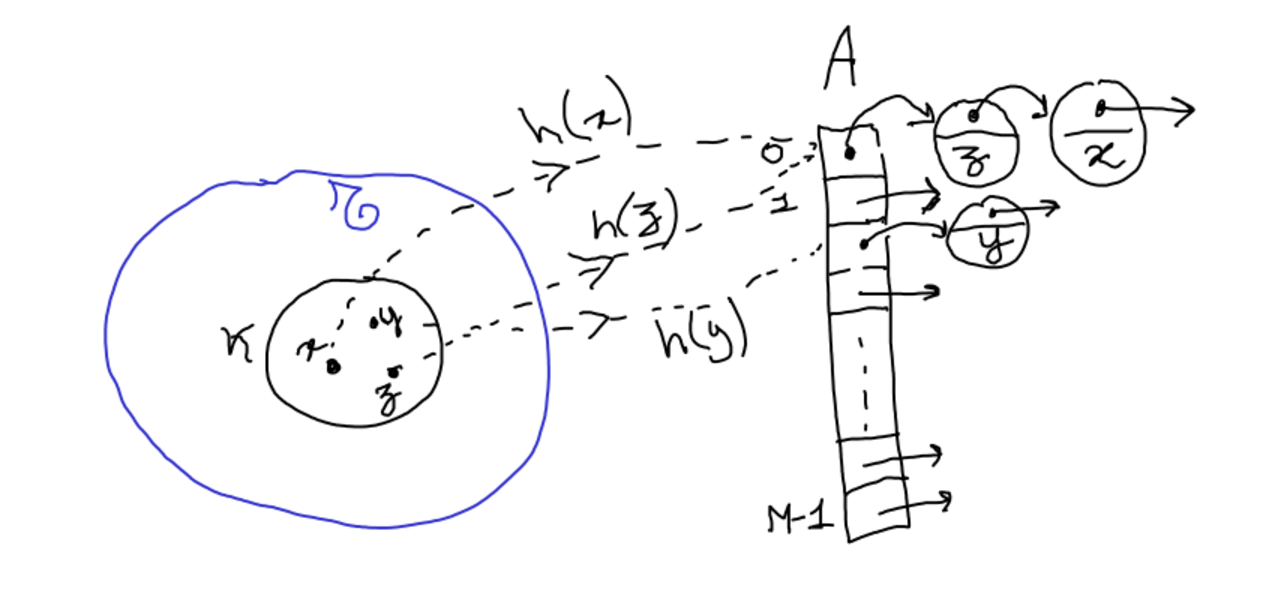
\includegraphics[width=14cm]{data/chaining.pdf}

This work-around is relatively easy to implement {\it if} we allow ourselves memory 
allocation on each new insert. It is also the easiest to analyze from a
theoretical point of view. In particular,
\begin{equation}\label{eq:chainingcost}
\text{look-up time } = O(\text{length of chain at the corresponding table
slot}).
\end{equation}

Later we will discuss a second work-around, open addressing, that avoids 
linked lists and allocations on each new insert. It generally leads to better
performance in practice, is also easy to implement, but is more complicated
to analyze from a theoretical standpoint. 

%%%%%%%%%%%%%%%%%%%%%%%%%%%%%%%%%%%%%%%%%%%%%%%%%%%%%%%%%%%%%%%%%%%%%%%%%%%%%%%
\subsection{What is a good hash function ?}
%%%%%%%%%%%%%%%%%%%%%%%%%%%%%%%%%%%%%%%%%%%%%%%%%%%%%%%%%%%%%%%%%%%%%%%%%%%%%%%

We should try to settle the following two questions~:
\begin{itemize}
	\item What is a good hash function ? In view of \eqref{eq:chainingcost}
		it should lead to as few collisions as possible (at least for
		pairs of keys in $\mathcal{K}$, if it is known prior to $h$, or
		for pairs of keys in $\mathcal{T}$ otherwise). It should also
		be fast to evaluate, as we already mentioned.
	\item What should be $M$ ? If we consider that $N$ is an input (the
		number of keys we must deal with) and $M$ is a design choice,
		then certainly we would like that $M$ is not too large with
		respect to $N$ (anything above $N$ can be considered as ``wasted
		space''. Typically, we could be pleased with $M = O(N).$ On the
		other end of the spectrum there is no minimal requirement if we 
		use chaining, $M$ could be chosen as small as $1$, but that
		would of course have implications on chains lengths and
		therefore on look-up time. So we should have in mind that $M$
		and $N$ should be of the same order.
\end{itemize}
	
To make clear the fact that the cost of evaluation of $h$ matters, here is an example 
of a hash function (assuming $\mathcal{K} = \{a_0,\cdots, a_{M-1}\}$ is known) that 
leads to zero collision (by construction!) over $\mathcal{K})$, but yet would be
a terrible choice :

\begin{lstlisting}[style=C]
/* T is an arbitrary type
 * a_0, ..., a_{N - 1} are constant literals of type T
 * is_equal implements equality on T x T 
 */
int bad_hash(T key)
{
	if (is_equal(key, a_0)) {
		return 0;
	} else if (is_equal(key, a_1)) {
		return 1;
	} else if (is_equal(key, a_2)) {
[...]
[...]
	} else if (is_equal(key, a_{N - 1})) {
		return (N - 1);
	} else {
		/* Don't care for keys out of K */
		return N;
	}
}
\end{lstlisting}

The elephant in the room is of course that evaluation of $bad\_hash$ is $O(N)$,
which annihilates the whole potential benefit of hashing.

\medskip
To minimize collisions, we have the intuitive idea that they keys should be
spread ``evenly'' by $h$. If we must choose $h$ before knowing $\mathcal{K}$
(the most common situation in applications), the we must deal with the following
bad news :

\begin{lemma} If $\#(\mathcal{T}) > (N-1)M$ then whatever hash function $h
	:\mathcal{T} \to {0, \cdots, M-1}$ is chosen, there exists an (unlucky)
	set of keys $\mathcal{K} \subset \mathcal{T}$ such that $\#(\mathcal{K})
	= N$ and all keys in $\mathcal{K}$ are hashed by $h$ to the exact same
	value.
\end{lemma}

In other words, there is no universally good hash function if the potential set 
of keys is too large with respect to the actual set of keys (which, in practice, 
will be the case almost all the time).

\begin{proof}
We may decompose
$$
	\mathcal{T} = \cup_{i \in \{0,\cdots, M-1\}} h^{-1}(i),
$$
where the union is disjoint by construction. In particular
$$
	\#(\mathcal{T}) = \sum_{i=0}^{M-1} \#(h^{-1}(i)).
$$
There must therefore exists at least some $0 \leq i_0 \leq M-1$ for
which
$$
	\#(h^{-1}(i_0)) \geq \frac{\#(\mathcal{T})}{M} > N - 1,
$$
	where we have used the assumption on $\#(\mathcal{T})$ for the last
	inequality. It suffices then to choose for $\mathcal{K}$ an arbitrary
	subset of $h^{-1}(i_0)$ of cardinality $N$.
\end{proof}

%%%%%%%%%%%%%%%%%%%%%%%%%%%%%%%%%%%%%%%%%%%%%%%%%%%%%%%%%%%%%%%%%%%%%%%%%%%%%%%
\subsection{Randomized hash functions and perfect hashing}
%%%%%%%%%%%%%%%%%%%%%%%%%%%%%%%%%%%%%%%%%%%%%%%%%%%%%%%%%%%%%%%%%%%%%%%%%%%%%%%

Although we have just seen that we cannot avoid black swans, we still wish to
devise hash functions that will try to efficiently spread keys evenly in the range
$0,\cdots M-1$. 

It is tempting to use some kind of randomness. Imagine for a second that
for each key, $h(key)$ is a random function equally distributed in ${0,\cdots,
M-1}$ and that $h(key_1)$ and $h(key_2)$ are independent whenever $key_1
\neq key_2.$ In such situation, we would have for the probability of collisions :
\begin{equation*}\begin{split}
	P\big(h(key_1) = h(key_2)\big) &= P\big(\cup_{i=0}^{M-1} \{h(key_1) = h(key_2) =
	i\}\big)\\
	&= \sum_{i=0}^{M-1} P\big(h(key_1) = h(key_2) = i\big),
\end{split}
\end{equation*}
and from the independence and uniform distribution assumptions
\begin{equation*}\begin{split}
	\sum_{i=0}^{M-1} P\big(h(key_1) = h(key_2) = i\big) &= \sum_{i=0}^{M-1}
	P\big(h(key_1)=i\big)P\big(h(key_2) = i\big)\\
	&= \sum_{i=0}^{M-1} \frac{1}{M^2} = \frac{1}{M}.
\end{split}
\end{equation*}

Somehow we deduce from the former analysis that the target we should set
ourselves is 
\begin{equation}\label{eq:goodhash}
	\forall key_1 \neq key_2 \in \mathcal{T}, P\big( h(key_1) = h(key_2)\big) \leq \frac{1}{M}.
\end{equation}

The elephant in the room with our previous tentative is that if $h(key)$ uses
randomness it is evaluation, then look-ups will be doomed because the evaluation
will turn up different at insertion and at look-up time. 

Rather than using randomness in the {\it evaluation} of $h(key)$, we will instead
use randomness in the {\it design} of $h$ (but for similar reasons as just above, we 
should end up using the same $h$ for all operations after is has been chosen).

In the sequel, we therefore let $\Omega \subset \{0,\cdots, M-1\}^\mathcal{T}$
be a set of potential hash functions (note that $M$ is fixed up-front). We also 
endow $\Omega$ with a probability $P$ (in practice, often the uniform
probability on $\Omega$). We shall say $(\Omega,P)$ is a {\it universal} family
of hash functions precisely
when \eqref{eq:goodhash} holds.

\medskip
We have

\begin{lemma}\label{lem:O1}
Assume that the hash function $h$ is picked in $\Omega$ according to
$P$, and that it is used to fill a hash table of size $M$ using chaining. 
Assume that this hash table is used for an arbitrary sequence of 
inserts/deletes/look-up operations which never lead to its total size 
$N$ growing over $N = cM$, where $c >0$ is an arbitrary but fixed
constant. Then the expectation according to $P$ of the average cost of 
each of these operations is $O(1)$. 
\end{lemma}

This result is main theoretical selling point of hash table, compared to 
the costs $O(log(N)$ or even $O(N)$ which we discussed earlier. Of course
it only holds in expectation, as we have seen that there cannot be a
satisfactory a priori guarantee for whatever fixed $h$. 

\begin{proof}
We analyze the cost of an insertion, the reasoning for deletions and look-ups
are very similar. We know that in the case of chaining the cost of an insertion is
proportional to the length of the chain at the corresponding table slot. That number equals 
the number of keys already in the table at that collide with the inserted key.
In expectation, and if the family from which $h$ is picked in universal, that
number is $O(N/M) = O(1)$ in view of the assumption $N \leq cM.$  
\end{proof}

\begin{remark} Note the subtlety in the above statement that in order for the number of
insert / delete / look-up operations to tend to infinity (that's the only 
framework where $O(1)$ is meaningful) and at the same time verify that $N \leq cM$ 
(while $M$ is fixed, it must pre-exist $\Omega$), it is necessary that
in the sequence of operations deletes compensate inserts in the long run. 
\end{remark}

\medskip
{\bf Examples of universal families :}
Assume that the elements $\mathcal{T}$ are fixed size and can be identified with  
a sequence $b_1 \cdots b_l$ of $l$ chunks each one composed of $B$ bits (and
therefore holding a value in the set $0,\cdots, 2^{B}- 1$). We fix a {\it prime} integer
$M > 2^B$. For each choice of multiplicative coefficients $m_1, \cdots, 
m_k \in \{0, \cdots M - 1\}^k,$ we define the hash function 
$$
h(b_1\cdots b_l) = \sum_{i=1}^l m_ib_i \text{ modulo } M.
$$
We pretend that endowed with the uniform probability over $\{0, \cdots M -
1\}^k$, this constitutes a universal family of hash functions. Indeed, let
$key_1 = b_1\cdots b_l$ and $key_2 = b_1'\cdots b_l'$ be distinct. In particular
there exists at least one $1 \leq i_0 \leq l$ for which $b_{i_0} \neq b_{i_0}'.$
The collision $h(key_1) = h(key_2)$ arises if and only if
$$
m_{i_0}\Big(b_{i_0} - b_{i_0}' \Big) = \sum_{i \neq i_0} m_i \Big(b_{i}' -
b_{i} \Big).
$$
Whenever the coefficients $m_i$ with $i \neq i_0$ are chosen, the right hand
side above is fixed (let's call it $c_{i_0}$) and we may rewrite the equation as
\begin{equation}\label{eq:infield}
m_{i_0}\Big(b_{i_0} - b_{i_0}' \Big) = c_{i_0}.
\end{equation}
By assumption $0 \leq b_{i_0}, b_{i_0}' \leq 2^{B} - 1 < M$, and $b_{i_0} \neq
b_{i_0}'.$ In particular $b_{i_0} - b_{i_0}' \neq 0 \ \text{mod } M.$ Since 
$M$ is prime (and therefore $\mathbb{Z}/(M\mathbb{Z}$ is a finite field),
equation \eqref{eq:infield} possesses one and only one solution $m_{i_0} \in
\{0, \cdots, M-1\}$, namely
$$
m_{i_0} = \Big(b_{i_0} - b_{i_0}' \Big)^{-1} c_{i_0}\quad \text{ mod } M, 
$$
where the inverse is intended for multiplication modulo $M.$ Since $m_{i_0}$ 
is chosen according to the uniform probability over $0,\cdots, M-1$, it follows
that
$$
P\Big( h(key_1)= h(key_2)\Big) = \frac{1}{M}.
$$
This shows that the family is universal. 


\medskip

In the same spirit as for Lemma  \ref{lem:O1}, and with essentially the same
proof, we have

\begin{lemma}
	Let $M$ be fixed, $(\Omega,P)$ we a universal family of hash functions,
	and let $\mathcal{K} \subset \mathcal{T}$ be such that $\#(\mathcal{K})
	= N.$ Then
	$$
	\mathbb{E}\Big(\text{number of colliding pairs in } \mathcal{K} \Big)
	\leq \frac{N(N-1)}{2M}.
	$$
	In particular, if $M > N(N-1)/2$ then
	$$
	P\Big(\text{no colliding pair in } K\Big) \geq 1 - \frac{N(N-1)}{2M} > 0.
	$$
\end{lemma}
\begin{proof}
The expectation being a linear quantity which does not depend on independence,
the first statement is again an immediate consequence of the definition of a
universal family. For the second one, let us call $C$ the number of colliding
pairs. That
$$
	\mathbb{E}(C) = \sum_{k \geq 0} k P(C = k) = \sum_{k \geq 1} k P(C = k)
	\geq \sum_{k \geq 1} P(C = k) = 1 - P(C = 0),
$$
from which the conclusion follows.
\end{proof}


In particular, if we take $M = N^2$ then $P(\text{no colliding
pair in } K) \geq \frac12$ and therefore if picking successively hash 
functions at random in $\Omega$ according to $P$ we will need in 
expectation two tries before finding one leading to no collision 
[recall indeed that if a test has a probability $p$ of success (a Bernoulli variable $\mathcal{B}(p)$) then the
the number of independent tries before the first success (a Geometric variable
$\mathcal{G}(p)$) has expectation $\frac{1}{p}$].

\medskip

But $M = N^2$ is disappointing in terms of space needed (we would
wish a table with $M = O(N)$ as anything above $N$ can be considered 
a waste of space with respect to the space needed for the mere data). 

\medskip

We shall resolve that issue using {\it double hashing}. Let indeed $(\Omega, P)$ be a
universal family of hash functions with the choice $M = N$. Pick a hash
function $h$ at random in $\Omega$ according to $P$, and denote  
$$N_i := \#(h^{-1}(i)), \text{ for } i = 0,\cdots M - 1 = N-1.$$
The previous lemma is of no use at the level of $h$, and we cannot hope the $N_i$ to be all
equal to 1 (that would correspond to a collision free hash). But for each given
$i$, using the previous analysis we can find (and even construct) a hash function $h_i$ (in a
corresponding universal hash family $(\Omega_i,P_i)$ based on $M \equiv N_i^2$)
into a table of size $N_i^2$ and such that 
$$
h_i(key_1) \neq h_i(key_2) \qquad \forall key_1 \neq key_2 \in h^{-1}(i).
$$
All these tables can be viewed as sub-arrays of a large array whose total size is $\sum_i N_i^2.$ The final hash
function is then
\begin{enumerate}
	\item compute $i := h(key)$
	\item place $key$ in the sub-array $i$ at position (within the
		sub-array) $h_i(key)$.
\end{enumerate}
By construction and by assumption on the $h_i$, this hash produces no collision
over $K$. It remains to evaluation the total size $\sum_i N_i^2.$
For that purpose, for $k1, k2 \in K$ let $C(k1,k2)$ denote the random variable
which is equal to one if $k1$ and $k2$ collide under $h$ and 0 otherwise. Then
it is straightforward to check that, pointwise as functions over $\Omega$, 
$$
\sum_{i=0}^{N-1} N_i^2 = \sum_{k1 \in K} \sum_{k2 \in K} C(k1,k2)
$$
In particular, taking expectations we obtain 
\begin{equation*}\begin{split}
\mathbb{E}(\sum_{i=0}^{N-1} N_i^2) &= \sum_{k1 \in K} \sum_{k2 \in K}
\mathbb{E}(C(k1,k2))\\
&= \sum_{k1 \in K}\mathbb{E}(C(k1,k1)) + \sum_{k1 \neq k2 \in
K}\mathbb{E}(C(k1,k2))\\
& \leq N + N(N-1)\frac{1}{M} = 2N - 1.
\end{split}\end{equation*}
Recall that for a non negative random variable $X$ and for any $c>0$, $P(X
\geq c) \leq \frac{\mathbb{E}(X)}{c}$ (this is called Markov inequality in
probability, and Tchebychev inequality in measure theory). If we apply it to 
$\sum_{i=0}^{N-1} N_i^2$ and $c= 4N$, we obtain
$$
P(\sum_{i=0}^{N-1} N_i^2 \geq 4N) \leq \frac{2N-1}{4N} \leq \frac12,
$$
or conversely that
$$
P(\sum_{i=0}^{N-1} N_i^2 \leq 4N) \geq \frac12. 
$$
As a consequence, if we pick the initial $h$ at random then after 2 tries in
expectation we shall find a one for which $\sum_{i=0}^{N-1} N_i^2 \leq 4N$, and
therefore for which the corresponding final aggregated hash table will have a size
less or equal to $4N = O(N)$, hence achieving our goal.  

\medskip

In many contexts though, the set of keys is not known prior to the choice of the
hash function, and it is hopeless to avoid having to deal with collisions. We
have seen how chaining can be used to deal with them. We mentioned that another
solution, which often turns out more performant in practice, will be discussed
later. This is our last goal for the section about hashing.

%%%%%%%%%%%%%%%%%%%%%%%%%%%%%%%%%%%%%%%%%%%%%%%%%%%%%%%%%%%%%%%%%%%%%%%%%%%%%%%
\subsection{Collision work-around \# 2 : open-addressing} 
%%%%%%%%%%%%%%%%%%%%%%%%%%%%%%%%%%%%%%%%%%%%%%%%%%%%%%%%%%%%%%%%%%%%%%%%%%%%%%%

In open addressing the hash table is exclusively based on an array, which means that
colliding keys will not be inserted into linked list located in each table
slot. Instead colliding keys will be dealt with by advancing in the table until
a free slot is found. More precisely, to insert a new key in the table :
\begin{enumerate}
	\item Compute {\tt pos = hash(new\_key)}
	\item While {\tt A[pos]} is occupied, increment {\tt pos} by by one and round
		the result modulo the table size (so that if we reach the end of
		the table we cycle back at the beginning of it).
	\item Finally insert the key at {\tt A[pos]} (the current value of {\tt
		pos}, not the original one).
\end{enumerate}

Of course this is only possible if the size of the hash table is at least as
large as the number of keys it needs to store (i.e. $M \geq N$ is our previous
notations), or the inserts will end-up cycling for ever without finding a free
slot.
$$
\text{The ratio } \frac{N}{M} \text{ is called the load factor of the table,}
$$
and it must remain smaller than one. In practice it is important to keep
a load factor sufficiently bounded away from 1 (e.g. $66\%$) or insertions
will start to become costly due to the potential large number of occupied slots 
encountered while resolving a collision.

\medskip

Care must also be taken regarding deletions. The naive solution would be to just
first find the key (following the same scheme as for inserts) and then deleting
it (marking the slot as empty again). This would unfortunately potentially break
later look-ups. Indeed, imagine the following sequence :
\begin{enumerate}
	\item Insert key {\tt k1} which hashes to position {\tt pos}.
	\item Insert key {\tt k2} which collides with {\tt k1} and ends-up
		inserted at position {\tt pos + 1}.
	\item Insert key {\tt k3} which collides with {\tt k1, k2} and ends-up
		inserted at position {\tt pos + 2}.
	\item Delete key {\tt k2}. Now the slot at position {\tt pos + 1} is
		marked as free.
	\item Look-up for {\tt k3}. It hashes to {\tt pos}, the slot is
		occupied, the next slot is checked and read as empty and
		therefore it is concluded that {\tt k3} is not present in the
		table, which is obviously wrong.
\end{enumerate}

To overcome this difficulty, the slots of the table will be marked either free,
occupied, or deleted. The slots marked deleted are jumped over when performing
look-ups, and instead they are considered as free slots when performing new
insertions.

\medskip

The following C code implements a dictionary (i.e. a set of distinct keys and
their corresponding associated values) using an open addressing hash table. In 
production implementations a number of improvements are usually adopted (briefly 
discussed below).

\begin{lstlisting}[style=C]
#ifndef _HASH_TABLES_H
#define _HASH_TABLES_H

// Implementation of a dictionary of (key,value) using
// a hash table based on open addressing.
// Genericity for key and value types is obtained by type
// erasure and use of memcmp and memcpy. Keys and values
// must therefore be of fixed length.

struct HashTable {
	unsigned capacity;  // Nbr of slots in the table
	unsigned size;	    // Nbr of occupied slots
	unsigned key_len;   // Size in bytes of each key
	unsigned val_len;   // Size in bytes of each value
	void *data;
};

void hash_table_init(struct HashTable *ht, unsigned capacity, unsigned key_len,
		     unsigned val_len);
void *hash_table_find(const struct HashTable *ht, void *key);
void hash_table_insert(struct HashTable *ht, void *key, void *val);
void hash_table_delete(struct HashTable *ht, void *key);
void hash_table_fini(struct HashTable *ht);

#endif
\end{lstlisting}


\begin{lstlisting}[style=C]
#include <stdint.h>
#include <stdlib.h>
#include <string.h>

#include "hash_tables.h"

#define FREE_SLOT 0
#define OCCUPIED_SLOT 1
#define DELETED_SLOT 2

void hash_table_init(struct HashTable *ht, unsigned capacity, unsigned key_len,
		     unsigned val_len)
{
	ht->capacity = capacity;
	ht->key_len = key_len;
	ht->val_len = val_len;
	ht->size = 0;
	unsigned slot_len = 1 + key_len + val_len;
	ht->data = malloc(capacity * slot_len);
}

/* A general purpose hash function : FNV-1a 32 bits. Cfr :
 * https://en.wikipedia.org/wiki/Fowler%E2%80%93Noll%E2%80%93Vo_hash_function
 */
uint32_t hash_key(void *key, unsigned key_len)
{
	unsigned char *byte = key;
	uint32_t hash = 2166136261;
	while (key_len--) {
		hash ^= *byte++;
		hash *= 16777619;
	}
	return hash;
}

void *hash_table_find(const struct HashTable *ht, void *key)
{
	uint32_t pos = hash_key(key, ht->key_len);
	unsigned slot_len = 1 + ht->key_len + ht->val_len;
	unsigned char *data = ht->data;
	while (1) {
		pos = pos % ht->capacity;
		unsigned char *p = data + pos * slot_len;
		if (p[0] == FREE_SLOT) {
			return NULL;
		}
		if (p[0] == OCCUPIED_SLOT &&
		    memcmp(key, p + 1, ht->key_len) == 0) {
			return p + 1 + ht->key_len;
		} else {
			pos++;
		}
	}
}

static void hash_table_grow(struct HashTable *ht, size_t new_cap)
{
	// Left as an exercise :
	// 1. Save the address ht->data for later use.
	// 2. Init a new table with new_cap capacity (that will 
	//    overwrite	ht->data)
	// 3. Traverse the old table, read its data and insert it
	//    (e.g. through hash_table_insert) into the new table.
	// 4. When done, free the old data
}


void hash_table_insert(struct HashTable *ht, void *key, void *val)
{
	if (ht->size >= 2 * ht->capacity / 3) {
		size_t new_cap = ht->capacity < 4 ? 8 : 2 * ht->capacity;
		hash_table_grow(ht, new_cap);
	}
	uint32_t pos = hash_key(key, ht->key_len);
	unsigned slot_len = 1 + ht->key_len + ht->val_len;
	unsigned char *data = ht->data;
	while (1) {
		pos = pos % ht->capacity;
		unsigned char *p = data + pos * slot_len;
		if (p[0] != OCCUPIED_SLOT) {
			memcpy(p + 1, key, ht->key_len);
			memcpy(p + 1 + ht->key_len, val, ht->val_len);
			p[0] = OCCUPIED_SLOT;
			return;
		} else {
			pos++;
		}
	}
}

void hash_table_delete(struct HashTable *ht, void *key)
{
	uint32_t pos = hash_key(key, ht->key_len);
	unsigned slot_len = 1 + ht->key_len + ht->val_len;
	unsigned char *data = ht->data;
	while (1) {
		pos = pos % ht->capacity;
		unsigned char *p = data + pos * slot_len;
		if (p[0] == FREE_SLOT) {
			return;
		}
		if (p[0] == OCCUPIED_SLOT &&
		    memcmp(key, p + 1, ht->key_len) == 0) {
			p[0] = DELETED_SLOT;
			return;
		} else {
			pos++;
		}
	}
}

void hash_table_fini(struct HashTable *ht)
{
	free(ht->data);
	ht->data = NULL;
	ht->capacity = ht->size = 0;
}

#undef FREE_SLOT
#undef OCCUPIED_SLOT
#undef DELETED_SLOT
\end{lstlisting}

As already mentioned  the previous implementation, although avoiding linked
lists, can be improved in a number of ways. 

\begin{enumerate}
	\item If the table size is required to be a power of two, then it is
		possible to replace the modulo operation by a bitwise operation (which even 
		on today's architecture is substantially less costly). Indeed,
		due to integer representation if $M$ is a power of two then
		modulo $M$ amounts to bitwise AND with $M - 1$ (think about it
		if it isn't immediately clear, $M-1$ in such a case is a
		sequence of zero bits followed by a sequence of one bits, as
		many as the correspond power of two $M$ is).
	\item The linear probing (that is the fact that if slot {\tt pos} is
		occupied we advance to {\tt pos + 1}) can be replaced by a quadratic 
		probing. The latter corresponds to advancing to {\tt pos +
		probe}, where {\tt probe} is the probe number. In other words,
		the first position checked if {\tt pos} is occupied is {\tt pos
		+ 1} (first probe). If is is also occupied we jump to {\tt pos +
		1 + 2} (second probe), etc to {\tt pos + 1 + 2 +... + k} until
		(say) we find a free slot at probe number k. Quadratic probing has the advantage that it 
		avoids clustering of occupied cells after collisions (it spreads
		new probes further away wrt linear probing). It must only be
		used when the first optimization above applies, i.e. with tables
		whose length is a power of two. The reason is that when $M$ is a
		power of two the mapping {\tt probe $\to$ pos  +
		probe(probe+1)/2 modulo M} induces a bijection from 
		$\{0,\cdots , M- 1\}$ into itself (this is not immediate, we did
		the proof in class but it isn't particularly enlightening, so I
		skip it here). For $M$ not a power of 2, it is generally not the
		case, and the table may then appear full to the algorithm
		(because not all cells would be visited by the jump process)
		although it isn't. 
	\item The occupancy status byte of each slot can be avoided by reserving
		(whenever possible) two keys in the set of all potential keys 
		to represent free and deleted slots. This not only saves one
		byte (which often isn't a big deal since keys and values generally
		occupy more than that) but often offers some alignment 
		optimizations to the compiler, especially with the next
		optimization.
	\item  Generic programming in C is convenient and acceptably fast, but
		type erasure (i.e. use of {\tt void*}  and {\tt memcpy, memcmp}
		prevent the compiler from potentially optimization possible when
		the type of the data is known at compile type. \cpp through the
		use of templates can be used to overcome this.
\end{enumerate}

The next \cpp code snippet shows all these optimizations working together in a hash
look-up function. The types of the keys (and values not shown here) are templates 
to be filled by the user at the time of the hash-table instantiation (we shall
discuss that in two weeks). The hashing is delegated to a hasher type (another
template parameter) which must implement, in addition to {\tt hash}, the {\tt
is\_equal} and {\tt is\_empty} functions. Note the look-up function does not
return a value here, but simply the index in the table (the user can read at that
slot index to decide what to do (insert/delete/whatever)).
	


\begin{lstlisting}[style=C]
template<typename K, typename H>
static inline size_t hash_lookup(K *keys, size_t buckets, H hasher, K key)
{
	/* In debug mode, assert the table size is indeed a power of two */
	assert(((buckets - 1) & buckets) == 0);
	
	size_t mask = buckets - 1;
	size_t bucket = hasher.hash(key) & mask;

	for (size_t probe = 0; probe < buckets; probe++) {

		if (hasher.is_empty(keys[bucket]) || 
				hasher.is_equal(keys[bucket], key)) {
			return bucket;
		}
		/* quadratic probing */
		bucket = (bucket + probe + 1) & mask;
	}
	
	/* Should never reach this point */
	assert(false && "Table is full !\n"); 	
	return 0;
}
\end{lstlisting}


%%%%%%%%%%%%%%%%%%%%%%%%%%%%%%%%%%%%%%%%%%%%%%%%%%%%%%%%%%%%%%%%%%%%%%%%%%%%%%%
%%%%%%%%%%%%%%%%%%%%%%%%%%%%%%%%%%%%%%%%%%%%%%%%%%%%%%%%%%%%%%%%%%%%%%%%%%%%%%%
\pagebreak
\section{Trees}
%%%%%%%%%%%%%%%%%%%%%%%%%%%%%%%%%%%%%%%%%%%%%%%%%%%%%%%%%%%%%%%%%%%%%%%%%%%%%%%
%%%%%%%%%%%%%%%%%%%%%%%%%%%%%%%%%%%%%%%%%%%%%%%%%%%%%%%%%%%%%%%%%%%%%%%%%%%%%%%


%%%%%%%%%%%%%%%%%%%%%%%%%%%%%%%%%%%%%%%%%%%%%%%%%%%%%%%%%%%%%%%%%%%%%%%%%%%%%%%
\subsection{Some definitions and generalities}
%%%%%%%%%%%%%%%%%%%%%%%%%%%%%%%%%%%%%%%%%%%%%%%%%%%%%%%%%%%%%%%%%%%%%%%%%%%%%%%

Let $V$ be a finite set, and $E \subseteq V \times V.$ The elements in $V$
are called vertices (or nodes) and those in $E$ are called edges. Whenever $e =
(v_1,v_2) \in E$, we say that $v_1$ is a parent of $v_2$, and that $v_2$ is a
child of $v_1$.

\begin{definition} 
$(V,E)$ is a rooted tree with root $r \in V$ if and only if
	\begin{enumerate}
		\item all nodes in $V \setminus \{r\}$ have exactly one parent.
		\item the root $r$ has no parent.
	\end{enumerate}
By convention, an empty set of nodes and edges is also called a rooted tree
(with no root). Nodes in the tree that have non children are called leaves.
\end{definition}

A number of easy properties or new definitions are in order :

\begin{itemize}
	\item
		For every $v \in V$, there exists a unique $n \in \N$ and a
		unique path
		$$
		r = e_0 \to e_1 \to \cdots \to e_n = v 
		$$
		such that for each $0 < i < n-1$, $(e_i,e_{i+1}) \in E$. The
		length $n$ of the path is called the depth of the node $v$. 
	\item
		By definition\footnote{Some authors prefer a different
		convention which differs by one, the empty tree having a height
		of $-1$} the height of a rooted tree is zero if it is empty
		or else one plus the largest depth among its nodes (or
		equivalently among its leaves) if not. It is therefore also the
		number of visited nodes in the longest path in the tree.
	\item   Given $v, w \in V$, $v$ is called an ancestor of $v$ if $w$ belongs to 
		the unique path joining the root to $w$.
		Inversely, $w$ is then called an descendent of $v$.
	\item   For $v \in V$, the {\it sub-tree rooted at $v$} is the tree which has 
		for vertex set $V' = \{
			v' \in V \text{ s.t. } v' \text{ is a descendent of }
			v\}$ and for edge set $E' = \{(v',w') \in E \text{ s.t. }
		v'\in V',\ w' \in V'\}$.
\end{itemize}

\begin{definition} 
A binary tree is a rooted tree for which each node as at most two children.
\end{definition}

Since there are at most two children per node in binary trees, it is common 
to think of their nodes as having two slots: one for the so-called left children and
the other for the so-called right children. These slots can be occupied or empty.
Accordingly, each node $v \in V$ possesses a (possibly empty) left sub-tree, 
noted $lst(v)$, and a (possibly empty) right sub-tree, noted $rst(v)$. These
sub-trees are respectively rooted at the left and right children of $v$, when 
the latter exist.

\medskip

Searching into trees will imply traversing them down from the root. In
applications, it is therefore desirable to keep their height under control. If a
tree contains $N = \#(V)$ nodes, then its height $H$ can be as large as $N - 1$
(when the tree is no more than an linked list). On the extreme opposite, if a
binary tree is perfect (i.e. if all its leaf nodes are at the same depth and all non 
leaf nodes have exactly two children), then $N = 1 + 2^1 + 2^2 + \cdots + 2^{H -
1} = 2^H - 1.$ In particular $H = \log_2(N + 1)$ for such trees. Perfect trees are often too
constrained to be useful. The following balanced trees will both be flexible
enough and have a sufficiently good upper bound on their height.

\begin{definition} A binary tree is called balanced if for each $v \in V$, the
	height of its left and right sub-trees differ at most by one.
\end{definition}
\begin{lemma}
If a binary tree is balanced, then its height $H$ and its total number
of nodes $N$ satisfy that
$$
	N \geq  F_{H + 1} + 1,
$$
	where $(F_k)_{k \geq 0}$ is the Fibonacci sequence : $F_0 = 0$, $F_1 =
	1$, and $F_{k} = F_{k - 1} + F_{k-2}$ for $k \geq 2.$\\
	In particular 
	$$H = O(\log N)$$
	as $N \to +\infty.$
\end{lemma}
\begin{proof}
	Let's call $T(h)$ the minimal number of nodes in a balanced binary tree of height
	$h \geq 0$. Clearly $T(0) = 0$, $T(1) = 1$, and for $h \geq 2$
	$$
	T(h) \geq 1 + T(h-1) + T(h-2).
	$$
	Indeed, the left and right sub-trees of the root must have heights equal
	to either $(h-1, h-1)$, or $(h-1, h-2)$ or $(h-2, h-1)$. Since $T$ is
	clearly increasing, the claimed inequality follows. If we note $S(h) =
	T(h) + 1$ then we obtain
	$$
	S(h) \geq S(h-1) + S(h-2) \qquad \forall h \geq 2,
	$$
	with $S(0) = 1$ and $S(1) = 2.$ It follows that $S(h) \geq F_{h+1}$, and
	hence the first claim in the statement. The Fibonacci sequence can be
	written in matrix form
	$$
	\begin{pmatrix} F_{k+1} \\ F_k \end{pmatrix} = 
		\begin{pmatrix} 1 & 1 \\ 1 & 0 \end{pmatrix} 
		\begin{pmatrix} F_{k} \\ F_{k-1} \end{pmatrix}, 
	$$
	and therefore also
	$$
	\begin{pmatrix} F_{k+1} \\ F_k \end{pmatrix} = 
		\begin{pmatrix} 1 & 1 \\ 1 & 0 \end{pmatrix}^k 
		\begin{pmatrix} F_{1} \\ F_{0} \end{pmatrix}. 
	$$
	The eigenvalues of the matrix in the above expression are given by
	$\lambda_\pm = \frac{1 \pm \sqrt{5}}{2}$ and therefore as $k \to
	+\infty$
	$$
	\frac{F_k}{ \lambda_+^{k}} \to c > 0
	$$
	(eigenvectors must be computed to obtain $c$ explicitly), which implies that
	$$
	log(F_k) = k\log(\lambda_+) + o(1) \text{ as } k \to +\infty,
	$$
	and the second claim follows as well.
\end{proof}

In the sequel we shall restrict our attention to two families of binary trees
that have important applications as data structures : binary search trees (BST)
and binary heaps.

%%%%%%%%%%%%%%%%%%%%%%%%%%%%%%%%%%%%%%%%%%%%%%%%%%%%%%%%%%%%%%%%%%%%%%%%%%%%%%%
\subsection{Binary search trees (BST)}\label{subsec:bst}
%%%%%%%%%%%%%%%%%%%%%%%%%%%%%%%%%%%%%%%%%%%%%%%%%%%%%%%%%%%%%%%%%%%%%%%%%%%%%%%

Binary search trees are important alternatives to hash-tables for storing keys
or key/value pairs. While keys were hashed into hash tables, keys shall be sorted
into binary search trees. More precisely : 

\begin{definition} 
A binary search tree is a binary tree for which each node is associated with a key
and the following BST condition holds : 
	\begin{enumerate}
		\item $\forall v \in V$, $\forall w \in lst(v)$, $w.key < 
			v.key$
		\item $\forall v \in V$, $\forall w \in rst(v)$, $w.key > 
			v.key$.
	\end{enumerate}
\end{definition}

In particular, keys must be distinct\footnote{Although, there are ways to
circumvent this limitation in practice, it is a good exercise to think about it}.

\medskip

Finding a key in a BST is therefore as simple as :

\begin{itemize}
	\item Start at the root.
	\item Go down the three by choosing the left of right sub-tree at each
		encountered node by comparing the looked-up key with 
		the key of the node.
	\item When a leaf node is reached then new node is inserted as its left
		or and the key has still not been found then it
		isn't in the tree.
\end{itemize}

Insertions are very similar : 

\begin{itemize}
	\item Start at the root.
	\item Go down the three by choosing the left of right sub-tree at each
		encountered node by comparing the key to be inserted with 
		the key of the node.
	\item Insert the key as a new node (which shall be a leaf) when the 
		are no more sub-tree to visit reaching an .
\end{itemize}


The following simple implementation is based on recursion. The values
here are assumed to be integers for simplicity. They might be replaced by any 
type together with an ordering.  In the tutorials, you will deal with a situation where
the tree nodes are contained in the data (this is called an intrusive tree), 
rather containing it, it is a much more common use in real applications, which
also has the advantage to delegate memory allocation to the user side.
Note also that in this implementation we allow nodes with equal values.

\begin{lstlisting}[style=C]
#include <stdlib.h>
#include <stdbool.h>

struct Node {
	int val;
	struct Node *child[2]; /* 0 = left, 1 = right */
};

static struct Node *new_node(int val)
{
	struct Node *n = malloc(sizeof(struct Node));
	n->val = val;
	n->child[0] = n->child[1] = NULL;
	return n;
}

struct Node *bst_find_recur(struct Node *root, int val)
{
	if (!root)
		return root;
	return bst_find_recur(root->child[val > root->val], val);
}

/* Note : In this implement duplicate vals are allowed */
struct Node *bst_insert_recur(struct Node *root, int val)
{
	if (!root) {
		root = new_node(val);
	} else {
		bool dir = val > root->val;
		root->child[dir] = bst_insert_recur(root->child[dir], val);
	}
	return root;
}
\end{lstlisting}

The case of deletions are slightly less obvious. In some implementations the
node is so-called ``lazy deleted'', which means it is marked as deleted but not
actually removed, and its key value is kept for later routing. Otherwise, the
proper way to do it is to swap the node to be deleted with either the smallest
node in its right sub-tree, or the largest node in its left sub-tree (and delete
the latter). There is a possible short-cut in the case where the node to be 
deleted only has one (or zero) children : in that case it suffices to deleted
the node and attach its (only or none) children to its grand parent. 

\begin{lstlisting}[style=C]
struct Node *bst_delete_recur(struct Node *root, int val)
{
	if (!root)
		return root;
	if (root->val != val) {
		bool dir = val > root->val;
		root->child[dir] = bst_delete_recur(root->child[dir], val);
	} else if (!root->child[0] || !root->child[1]) {
		bool dir = !root->child[0];
		struct Node *tmp = root->child[dir];
		free(root); /* might be null */
		root = tmp;
	} else {
		/* Smallest node in the root right sub-tree */
		struct Node *tmp = root->child[1];
		while (tmp->child[0]) {
			tmp = tmp->child[0];
		}
		/* Steal it */
		root->val = tmp->val;
		root->child[1] = bst_delete_recur(root->child[1], tmp->val);
	}
	return root;
}
\end{lstlisting}

The following variants avoid the use of recursion, this can be more efficient when
the tree becomes deeper. The lack of recursion implies that equivalent of parent
pointers must be kept and updated during the traverse down.

\begin{lstlisting}[style=C]
struct Node *bst_find(struct Node *root, int val)
{
	struct Node *n = root;
	while (n && n->val != val) {
		n = n->child[val > n->val];
	}
	return n;
}

struct Node *bst_insert(struct Node *root, int val)
{
	struct Node *nn = new_node(val);
	if (!root) {
		return nn;
	}

	struct Node *n = root;
	int dir = val > n->val;

	while (n->child[dir]) {
		n = n->child[dir];
		dir = val > n->val;
	}

	n->child[dir] = nn;
	return root;
}

struct Node *bst_delete(struct Node *root, int val)
{
	struct Node *del = root;  /* node to delete */
	struct Node *pdel = NULL; /* parent of node to delete */
	int dir;
	while (del && del->val != val) {
		dir = val > del->val;
		pdel = del;
		del = del->child[dir];
	}
	if (!del)
		return root;

	struct Node *rep; /* replacement node */
	if (!del->child[0]) {
		rep = del->child[1];
	} else if (!del->child[1]) {
		rep = del->child[0];
	} else {
		rep = del->child[1];
		struct Node *prep = del; /* parent of replacement node */
		while (rep->child[0]) {
			prep = rep;
			rep = rep->child[0];
		}
		if (prep != del)
			prep->child[0] = rep->child[1];
	}
	if (del != root) {
		pdel->child[dir] = rep;
	} else {
		root = rep;
	}
	free(del);
	return root;
}
\end{lstlisting}

\medskip
{\bf Average time complexity.} It is clear from the implementations that the costs of 
lookups/insert/delete are directly proportional to the height of
the tree. If the tree ends-up being very unbalanced (e.g. if the keys are inserted in
order or in reverse order, leading to a height $H = N- 1$), there will be no
advantage of a tree over a list. The following theoretical result shows that
in the mean (i.e. averaging over all possible shuffling of the input keys),
insertion costs are logarithmic.

\medskip

First, without loss of generality we can assume that set of keys to be inserted
are the integers $\{1, \cdots, N\}.$ Indeed, the actual keys do not matter,
only their ordering is important. Our averaging set will therefore be the set
$\sigma_N = \left\{ \sigma : \{1, \cdots, N\} \to \{1, \cdots, N\} \text{ a
permutation}\right\}$, equipped with uniform probability.

\begin{lemma}
The expectation of the total insertion cost of all the keys starting
from an empty BST is $O(N\log N)$.
\end{lemma}

As a consequence, the average cost per inserted key is $O(\log N)$. 

\medskip

By total insertion cost, we mean here the total number of comparisons  
(i.e. of routing) necessary for the whole process. 

\begin{proof}
	The key observation in order to count the number of comparisons during
	insertions is the following claim :\\
	{\bf Claim 1.} Let $1 \leq i < j \leq N$.  The keys $i$ and $j$ are compared at
	most once during the whole process, and they are compared if and
	only if there does not exist $i < k < j$ such that $\sigma(k) <
	\sigma(i)$ and $\sigma(k) < \sigma(j).$ 

	Indeed, first notice that $i$ and $j$ can only be compared during the insertion 
	of the one of the two that is inserted last (i.e. the one which has the largest 
	value under $\sigma$). Next, the keys are be compared if and only if
	they were not already sent into two different sub-trees by an earlier inserted 
	key. By the BST property, such a dividing key can only be of the form 
	$k$ with $i < k < j,$ which proves the claim.

	{\bf Claim 2.} Let $1 \leq i < j \leq N.$ Then the probability (according
	to $\sigma_N$ equipped with the uniform probability) that there exist no
	$i < k < j$ such that $\sigma(k) < \sigma(i)$ and $\sigma(k) <
	\sigma(j)$ is equal to $2/(j-i+1).$ 

	Indeed, by symmetry, among the $j-i+1$ numbers $i, \cdots, j$, all have the same
	probability (thus equal to $1/(j-i+1)$) to be the one which as the smallest 
	value under $\sigma$ . Therefore the probability that the one with the
	smallest value of $\sigma$ within $i,\cdots,j$ is either $i$ or $j$ is
	exactly $2/(j-i+1),$ which proves the second claim.

	Now the expectation of the total insertion cost is, by linearity of
	expectation :
	$$
	\sum_{i < j} \frac{2}{j-i+1}.
	$$
	We can compute the previous sum explicitly : 
	\begin{equation*}\begin{split}
		\sum_{i = 1}^{N-1} \sum_{j=i+1}^N \frac{2}{j-i+1} &=
		\sum_{i=1}^{N-1} \sum_{k=2}^{N-i+1} \frac{2}{k} = \sum_{k=2}^{N}
		\sum_{i = 1}^{N-k+1} \frac{2}{k} = \sum_{k=2}^N
		\frac{2(N-k+1)}{k}\\
		&= 2(N+1) \sum_{k=2}^N \frac{1}{k} - 2(N-1) = 2(N+1)\sum_{k=1}^N
		\frac{1}{k} - 4N.
	\end{split}\end{equation*}
	In the above, we have used the change of unknown $k = (j-i+1)$ in the
	first equality and the Fubini theorem for series for the second
	equality, the remaining ones being straightforward.  
	Since the harmonic series $\sum_{k=1}^N \frac{1}{k}= \log(N) + O(1)$ as $N \to
	+\infty$, the conclusion follows. 
\end{proof}

It can also be proved, but it is less immediate, that under the same setting the
expectation of the height of the BST after insertion is also of order $\log(N).$
This information is of similar nature but is not equivalent to the total
insertion cost. 

%%%%%%%%%%%%%%%%%%%%%%%%%%%%%%%%%%%%%%%%%%%%%%%%%%%%%%%%%%%%%%%%%%%%%%%%%%%%%%%
\subsection{Self balancing BST}\label{subsec:sb}
%%%%%%%%%%%%%%%%%%%%%%%%%%%%%%%%%%%%%%%%%%%%%%%%%%%%%%%%%%%%%%%%%%%%%%%%%%%%%%%

Although the average time complexity for insertions has been shown to be
$O(\log(N)$ in average, if we are unlucky the total cost could be as bad as $N$.
For that reason, our goal in this section is to present a modification of the
insertion and deletion processes that will have the following features : 
\begin{itemize}
	\item They are compatible with the BST property.
	\item They have (together with lookups) a guaranteed time complexity 
		of $O(\log N)$ where $N$ is the number of nodes in the tree at
		the time of the insertion/deletion/lookup. 
\end{itemize}

The key modification is a number of so-called rotations of the tree after an
insertion or a deletion in order to maintain a balanced tree. If this property
can be maintained, then we already know that the tree height will be  
$O(\log(N))$ and therefore so will be the cost of insertions/deletions/lookups.

\medskip

Rotations are described in the following figure : 

\begin{center}
	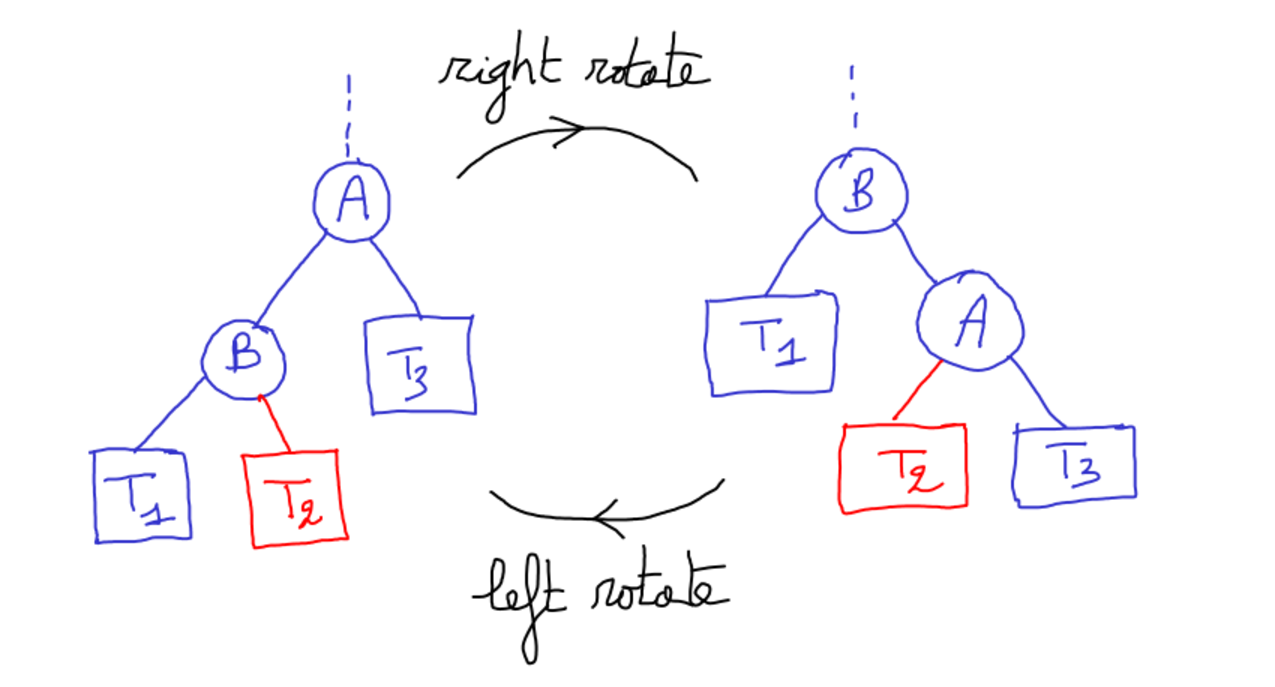
\includegraphics[width=14cm]{data/rotation.pdf}
\end{center}

In this figure, the round shapes represent tree nodes, while the square shapes
represent their (potentially empty) left of right sub-trees. During rotation, 
the node $A$ and $B$ exchange their parent/child relation. Since the one that
becomes the new parent can only keep at most two children (to remain a binary
tree), it must detach one of its sub-trees and reattach it to the one that
becomes a child. There is only one of such sub-trees that can be exchanged
($T_2$ in the figure) in order to maintain the BST property : all the 
nodes in $T_2$ are larger (in the sense of their key value) than $B$ and smaller
than $A$, both before and after the rotation. 

\medskip

It remains to explain how to maintain a balanced tree using rotations after an
insertion or a deletion. The first observation is that if the tree was balanced
before the insertion/deletion, the balance factors of the nodes in the tree after the
operation can only belong to the set $\{-2, -1, 0, 1, 2\}.$  Indeed, sub-trees
heights are modified at most by one unit when inserting or deleting a node.
Among these cases, only the ones with balance factors $\pm 2$ require some
rebalancing. In the sequel we assume therefore that some node in the tree, let's
call it $A$, has a balance factor $\pm 2$. We also assume that $A$ has the biggest 
depth among the unbalanced nodes (the other ones shall be treated after). By
symmetry, we can also assume that the balance factor of $A$ is $+2$, the case
$-2$ being perfectly left/right symmetrical.
Since the balance of $A$ is positive, the node $A$ must necessarily have a right
child, let's call it $B$. We shall distinguish two cases depending on the
balance factor of $B$ (by assumption $B$ is balanced since it has higher depth
than $A$).

\medskip

{\bf Case 1 :} The balance factor of $B$ is non negative.


In tat case we perform a single right rotation as in the figure below :


\begin{center}
	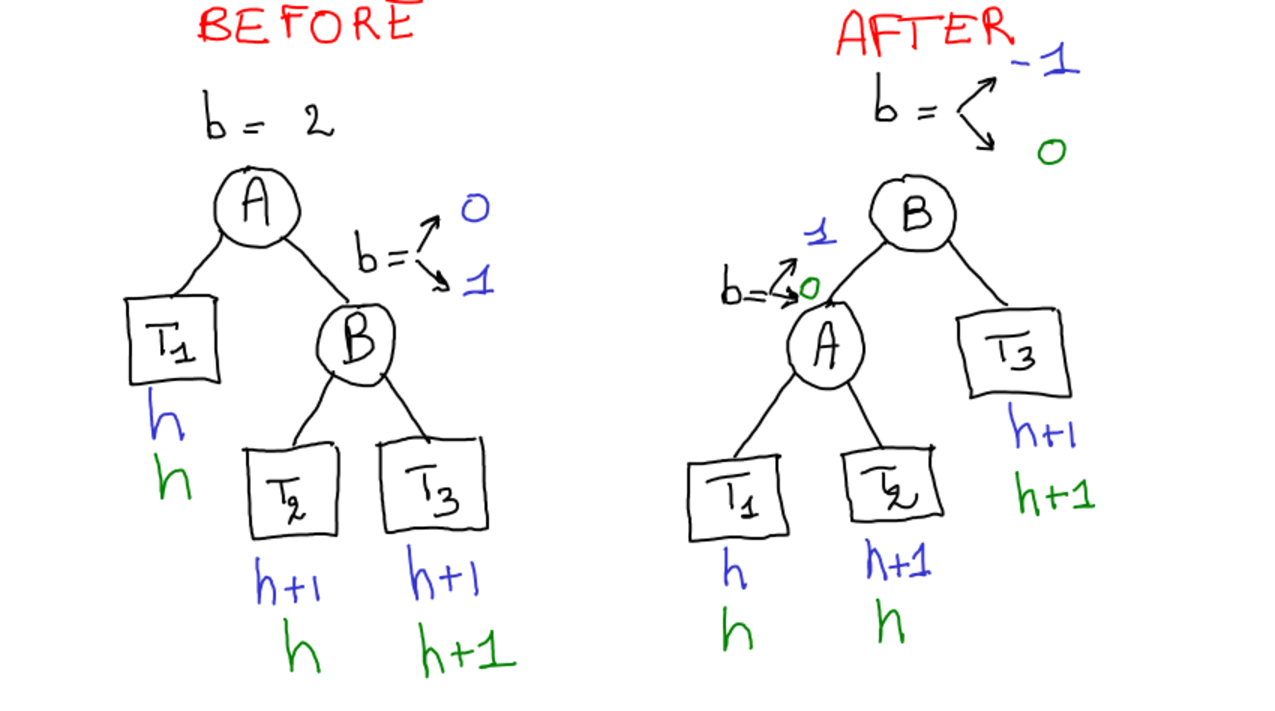
\includegraphics[width=14cm]{data/rebalance_simple.pdf}
\end{center}

We have noted $h$ the height of the left sub-tree of $A$ ($T_1$), the other
sub-tree heights have been deduced depending on the balance factor of $B$. 
We observe that after rotation, both $A$ and $B$ are balanced. 

Note also that only the green case can occur after an insertion leading to an
unbalance. Indeed, in the blue case the sub-trees $T_2$ and $T_3$ both have a
height $h+1$, and therefore at least one of them had a height of $h+1$ before
the insertion and then unbalance would have already been present. The
consequence of this is that the height of the tree rooted  at $B$
after rotation is exactly the same (i.e. $h+2$) as the height of the tree
rooted at $A$ before rotation and before the insertion took place 
(i.e. when $T_3$ had height $h$ and not $h+1$). This implies that the balance
factor of the nodes higher up in the tree are unaffected by the insert, and
therefore that {\bf at most one node can be unbalanced after an insertion
leading to Case 1}.
The same applies for deletions, except that both the blue and green cases can
occur. In the blue case both the tree after rotation and the tree before deletion 
(i.e. for which $T_1$ had height $h+1$) have total height $h+3$, while in the
green case they both have height $h+2$. Therefore {\bf at most one node can become 
unbalanced after a deletion leading to Case 1.}.

\medskip

{\bf Case 2 :} The balance factor of $B$ is negative (and hence $-1$).


In that case we perform a double rotation as in the figure below. Note that
since $B$ is left heavy, it must have a left child which we call $C$.


\begin{center}
	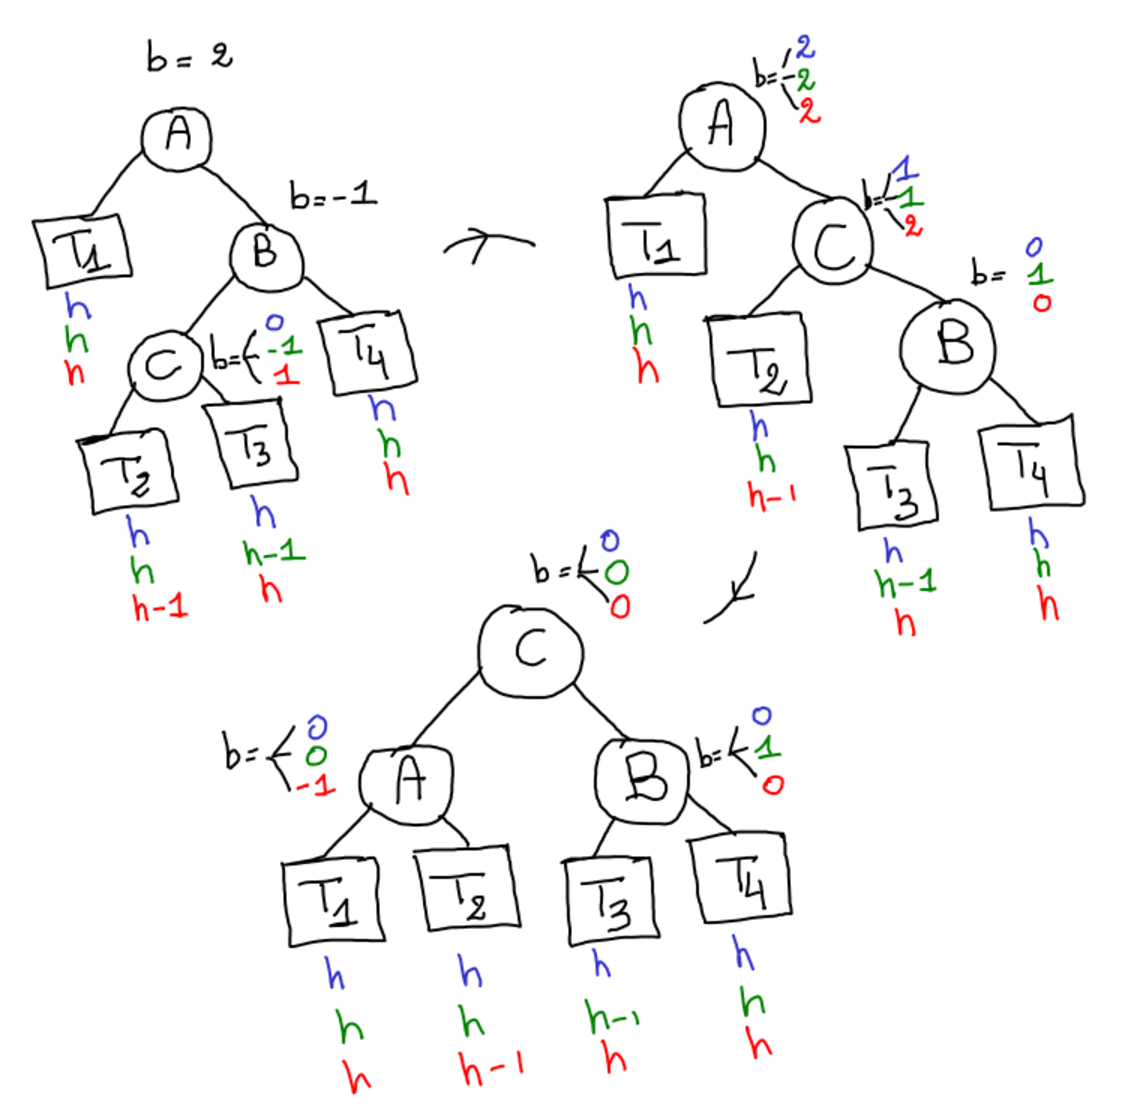
\includegraphics[width=14cm]{data/rebalance_double.pdf}
\end{center}

Here also we noted $h$ the height of the left sub-tree of $A$, and deduced the
other possible heights based on the balance factors. In the three colored cases,
the height of the tree rooted at $C$ after the double rotation is always 
$h + 2$.  Similar reasoning as above leads to the following :  only the green
and the red cases can occur for insertions, and they correspond to situations
where prior to insertion the height of the tree rooted at $A$ was $h+2$. Hence
the total height of the tree does not change after insertion + rebalancing, and
therefore {\bf at most one node can be unbalanced after an insertion
leading to Case 2}. The three colored cases can occur for deletions (i.e. when 
$T_1$ had height $h+1$ prior to deletion), but here the height of the tree
before deletion was different and equal to $h+3$, so we cannot unfortunately
conclude that rebalancing will occur only at one node for deletions. However,
the only nodes that can necessitate rebalancing are the ones along the path from
the root to the deleted nodes, and these are at most $O(\log(N))$ since the tree
is balanced.

\medskip

The trees which are maintained balanced following the above procedure are called
AVL trees (abbreviation for their inventors G. Adelson-Velsky and E. Landis).
Summarizing we have :

\begin{proposition}
	The cost for insertions/deletions/lookups in an AVL tree is always
	$O(\log(N))$, where $N$ is the number of nodes present in the tree.
	After an insertion, at most one node may necessitate rebalancing.
\end{proposition}

We finish this section with an extension of our previous implementation of BST
to the case of AVL.

\begin{lstlisting}[style=C]
#include <assert.h>
#include <stdlib.h>

struct AVLNode {
	int val;
	struct AVLNode *child[2]; /* 0 = left, 1 = right */
	int height; /* Height of the tree rooted at this node */
};

static struct AVLNode *new_node(int val)
{
	struct AVLNode *n = malloc(sizeof(struct AVLNode));
	n->val = val;
	n->height = 1;
	n->child[0] = n->child[1] = NULL;
	return n;
}

static int get_balance(struct AVLNode *root)
{
	if (!root)
		return 0;
	int left = root->child[0] ? root->child[0]->height : 0;
	int right = root->child[1] ? root->child[1]->height : 0;
	return right - left;
}

static void update_height(struct AVLNode *root)
{
	if (!root)
		return;
	int left = root->child[0] ? root->child[0]->height : 0;
	int right = root->child[1] ? root->child[1]->height : 0;
	root->height = 1 + (left > right ? left : right);
}

/* dir : 0 (false) = left, 1 (true) = right */
static struct AVLNode *rotate(struct AVLNode *root, bool dir)
{
	assert(root);
	struct AVLNode *next_root = root->child[!dir];
	assert(next_root);
	struct AVLNode *tmp = next_root->child[dir];
	root->child[!dir] = tmp;
	next_root->child[dir] = root;
	update_height(root);
	update_height(next_root);
	return next_root;
}

struct AVLNode *fix_balance(struct AVLNode *root)
{
	int b = get_balance(root);
	if (abs(b) <= 1)
		return root;
	/* dir = heavy direction = ! rotate direction */
	bool dir = b > 0;
	int b2 = get_balance(root->child[dir]);
	bool dir2 = b2 > 0;
	if (b2 && (dir != dir2))
		root->child[dir] = rotate(root->child[dir], !dir2);
	root = rotate(root, !dir);
}

struct AVLNode *avl_find(struct AVLNode *root, int val)
{
	if (!root)
		return NULL;
	return avl_find(root->child[val > root->val], val);
}

struct AVLNode *avl_insert(struct AVLNode *root, int val)
{
	if (!root) {
		root = new_node(val);
	} else {
		bool dir = val > root->val;
		root->child[dir] = avl_insert(root->child[dir], val);
		update_height(root);
		root = fix_balance(root);
	}
	return root;
}

struct AVLNode *avl_delete(struct AVLNode *root, int val)
{
	if (!root)
		return NULL;
	if (root->val != val) {
		bool dir = val > root->val;
		root->child[dir] = avl_delete(root->child[dir], val);
	} else if (!root->child[0] || !root->child[1]) {
		bool dir = !root->child[0];
		struct AVLNode *tmp = root->child[dir];
		free(root); /* might be null */
		root = tmp;
	} else {
		/* Smallest node in the root right subtree */
		struct AVLNode *tmp = root->child[1];
		while (tmp->child[0]) {
			tmp = tmp->child[0];
		}
		/* Steal it */
		root->val = tmp->val;
		root->child[1] = avl_delete(root->child[1], tmp->val);
	}
	if (!root)
		return NULL;
	update_height(root);
	root = fix_balance(root);
	return root;
}
\end{lstlisting}

%%%%%%%%%%%%%%%%%%%%%%%%%%%%%%%%%%%%%%%%%%%%%%%%%%%%%%%%%%%%%%%%%%%%%%%%%%%%%%%
\subsection{Binary heaps (and Heap sort)}
%%%%%%%%%%%%%%%%%%%%%%%%%%%%%%%%%%%%%%%%%%%%%%%%%%%%%%%%%%%%%%%%%%%%%%%%%%%%%%%

\begin{definition}
	A (max on top) binary heap is a rooted binary tree where each node is associated with 
	key and the following heap property holds :
	\begin{enumerate}
		\item $\forall v \in V$, $\forall w \in lst(v)$, $w.key <=
			v.key$.
		\item $\forall v \in V$, $\forall w \in rst(v)$, $w.key <=
			v.key$.
	\end{enumerate}
\end{definition}

By reversing all inequalities in the definition we would obtain a (min on top)
binary heap. The theory for both being completely parallel, it is common to
restrict to one of them. 

\medskip

In a sense, the heap replaces the left to right ordering of BST by a top to
bottom ordering. This change is more profound than it looks at first, in
particular one cannot easily perform a lookup of a key in a heap, because
there is no routing rule which can tell us whether to search in the left or
right child (we just know the keys in both sub-trees are smaller or equal to the
key at the visited node). For insertion, on contrary the freedom is greater,
since the heap property only tells us if we need to proceed down, but if yes we
can proceed left or right as we please. As a matter of fact, heap type data 
structures generally only implement lookup or extraction of the highest key, that is the one at the
root, and insertion of an arbitrary key (also, contrary to BST, keys in heaps may
not be unique). Heaps are typically used for implementing priority-queues, where extraction
of the task with highest priority is the only deletion op available, while
tasks of arbitrary priorities can be inserted.

\medskip

Because there is more freedom during insertion in heaps, the resulting tree can
be chosen to not only be balanced but also complete and full on the left. This means 
that all depth levels in the binary tree are full except possibly the one, 
corresponding to the highest depth, and which must only be full from the left.
An example is illustrated in the next figure :

\begin{center}
	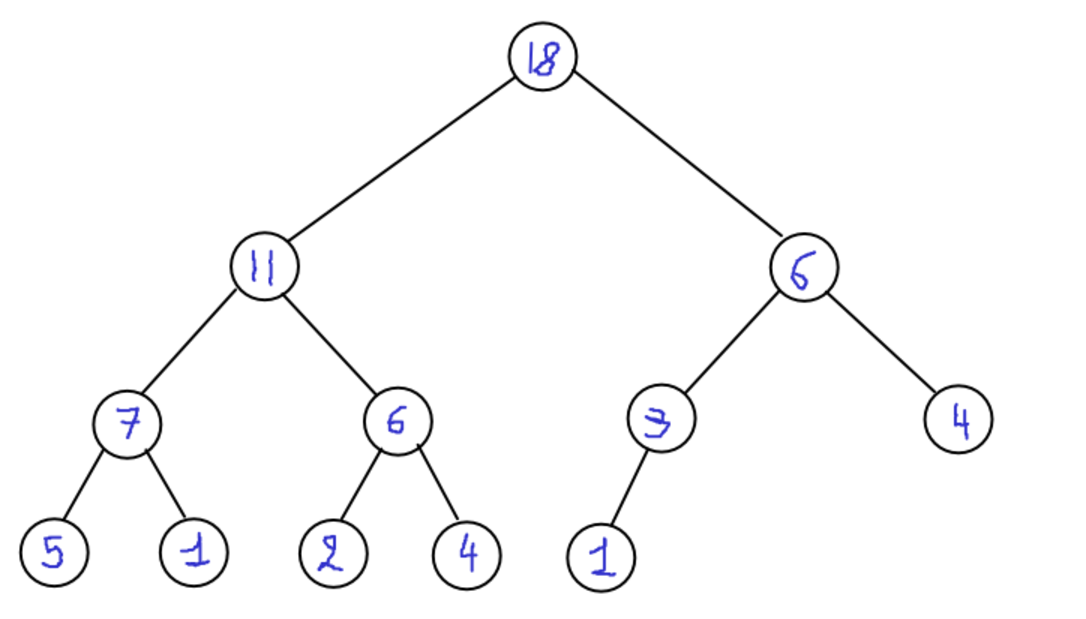
\includegraphics[width=14cm]{data/heap1.pdf}
\end{center}

Under this restriction, the position of of a newly inserted node is completely
constrained  and must occur at the ``lower-right'' position in the tree. Since
this may break the heap property, the newly inserted node is swapped with its 
parent in the tree as long as the heap property is not satisfied : this is
called a {\it sift-up} of the node. The next figure illustrate the result of
this process after a new node of value 10 as been inserted in the heap. 

\begin{center}
	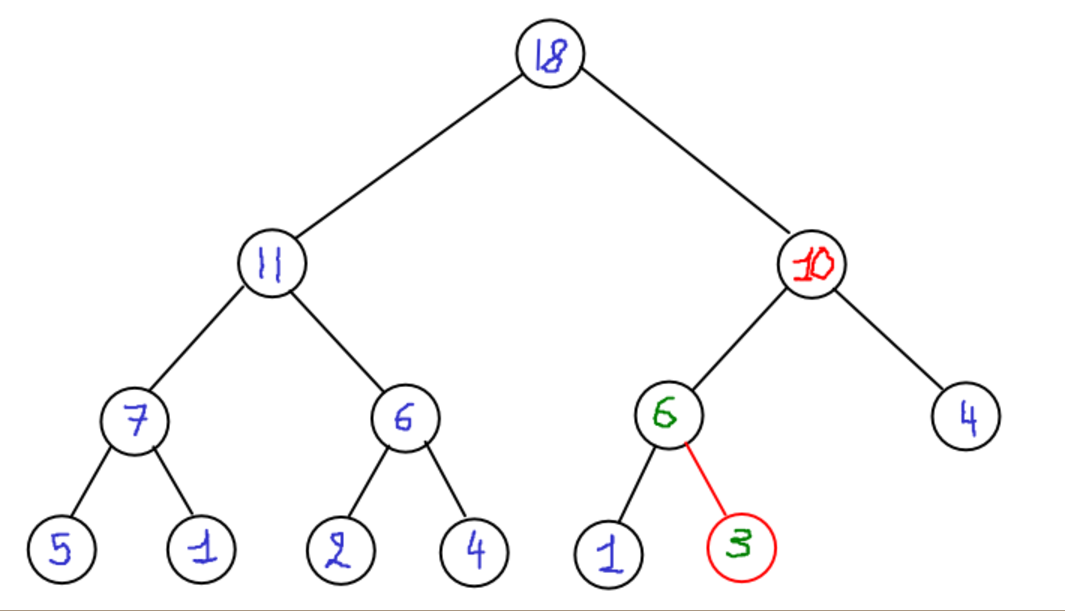
\includegraphics[width=14cm]{data/heap2.pdf}
\end{center}

When extracting the root node, the constraint to be a complete tree forces the
``lower-right'' node in the tree to moved in place of the old root. This again
breaks the heap property and the new root must be pushed down a number of time
in order to reset it. The correct governing rule for the push down is to swap
the node with the one of its two children which has the highest value (choosing
the one with the lowest value may imply another failure of the heap property),
as long as the heap property isn't satisfied. This is again illustrated in the
last figure below, we the heap is shown after the root 18 was extracted :

\begin{center}
	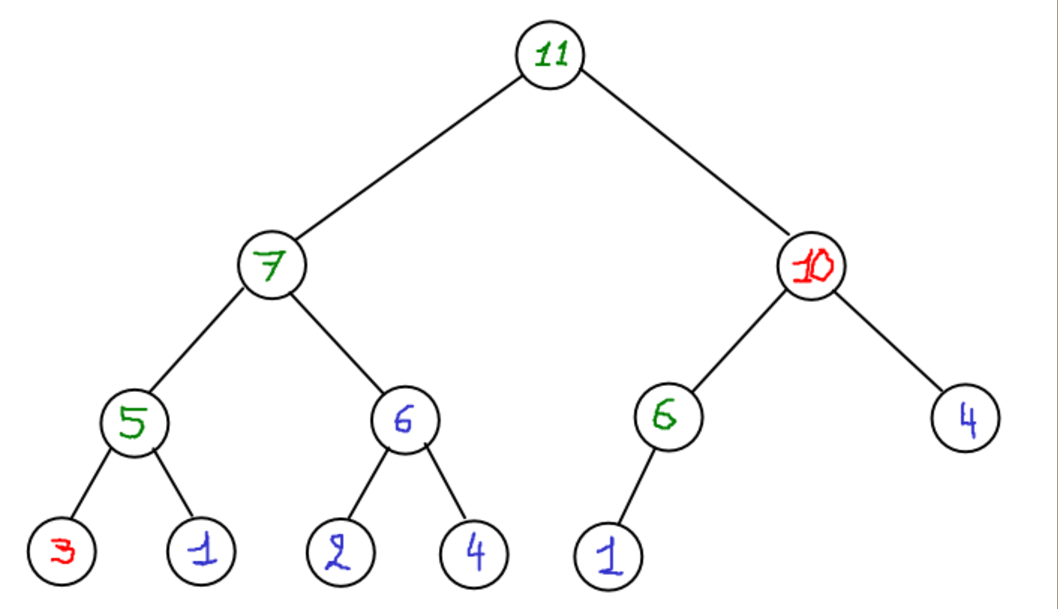
\includegraphics[width=14cm]{data/heap3.pdf}
\end{center}

The most interesting feature concerning this restriction about the tree to be a 
complete tree is that that such trees can easily be implemented as arrays, thus
avoiding the use of pointers and allocation at each insertion. In this array
implementation, the root node is placed at index 0, and the next indices in 
the array correspond to reading the tree from top to bottom and on each depth
level from left to right. Under this rule, the child-parent relation  
translates into the following simple expressions where $i$ refer to indices in
the array :
\begin{itemize}
	\item
		{\tt parent(i) = (i - 1) / 2}
	\item {\tt left\_child(i) = 2 * i + 1}
	\item {\tt right\_child(i) = 2 * i + 2}
\end{itemize}

The cost if insertion or extraction of the root in a heap, as in the case of
balanced tree, is $O(\log(N))$. This cost correspond to the maximum number of
swaps which occur during each of such operations, and is bounded by the total height of
the tree, which is $O(\log(N))$.

The $C$ code for such implementations is the object of one of the tutorials,
with an additional feature to allow for node value update, which will be helpful
when implementing the Dijkstra algorithm for finding optimal paths in weighted graphs.

%%%%%%%%%%%%%%%%%%
%TODO : Heap sort
%%%%%%%%%%%%%%%%%%

%%%%%%%%%%%%%%%%%%%%%%%%%%%%%%%%%%%%%%%%%%%%%%%%%%%%%%%%%%%%%%%%%%%%%%%%%%%%%%%
%%%%%%%%%%%%%%%%%%%%%%%%%%%%%%%%%%%%%%%%%%%%%%%%%%%%%%%%%%%%%%%%%%%%%%%%%%%%%%%
\pagebreak
\section{Graphs}
%%%%%%%%%%%%%%%%%%%%%%%%%%%%%%%%%%%%%%%%%%%%%%%%%%%%%%%%%%%%%%%%%%%%%%%%%%%%%%%
%%%%%%%%%%%%%%%%%%%%%%%%%%%%%%%%%%%%%%%%%%%%%%%%%%%%%%%%%%%%%%%%%%%%%%%%%%%%%%%

\begin{definition}A graph $G=(V,E)$ is given by a set $V$, whose elements are
called the vertices (or the nodes) or the graphs, and 
a subset $E \subseteq V \times V$, whose elements are called the edges of the
graph. \end{definition}

In the sequel, we shall always implicitly assume, whenever we consider a graph
$G=(V,E)$, that the set $V$ (and hence $E$) is a finite set. The notations $|V|$ 
and $|E|$ will be used to refer to the cardinality of $V$ and $E$ respectively, 
and when this is convenient we shall label the vertices in $V$ from $1$ to $|V|.$

Since $E \subseteq V \times V$ it always holds that $0 \leq |E| \leq |V|^2.$ 
A graph is called sparse if $|E|$ is ``much smaller'' than $|V|^2$, and many 
important cases we have $|E| = O(|V|)$ (in particular when the {\it degree}  
of each vertex, that is the number of incoming edges into that vertex, is
bounded a priori). 

\medskip

Also since $E \subseteq V \times V$, the listing order
of an edge end-points matters, and for that reason graphs with the
abode definition are often called {\it directed} graphs. A graph is called {\it
undirected} if for all $(v,v') \in E$, the reverse edge $(v',v)$ also belongs to
$E.$

%%%%%%%%%%%%%%%%%%%%%%%%%%%%%%%%%%%%%%%%%%%%%%%%%%%%%%%%%%%%%%%%%%%%%%%%%%%%%%%
\subsection{Graph representation}
%%%%%%%%%%%%%%%%%%%%%%%%%%%%%%%%%%%%%%%%%%%%%%%%%%%%%%%%%%%%%%%%%%%%%%%%%%%%%%%

Often in implementation, once the vertex set $V$ is given, the edge set is not 
described as an abstract set of edges but using one or the other 
of the following two structures : 

\medskip

{\bf i) The adjacency matrix} This is the square $|V| \times |V|$ matrix $A$ for which
$$
A_{ij} = 1 \text{ if } (i,j) \in E \text{ else } 0.
$$
With this representation, the graph is undirected if and only if the adjacency
matrix is symmetric. The advantage of this representation is that it allows for
easy modification of the connectivity (i.e. adding or removing edges), since it
only amounts to changing some values between 0 and 1. The disadvantage of that 
representation is that it requires $O(|V|^2)$ memory. For sparse graphs, it
therefore represents a substantial waste of space (the matrix is sparse, in the
sense that it mostly contain zeros), and this is the reason why the second
representation below is favoured in such cases. As a matter of fact, in
scientific computing a number of important spare graphs come from sparse
matrices (e.g. the matrices used in solving partial differential equations using
finite differences or finite elements), and such matrices, are encoded using some 
a variation of the representation below.

\medskip

{\bf ii) The adjacency lists} In that case, for each vertex $i$ ($1 \leq i
\leq |V|$) the list
$$
Adj(i) := \left\{ i \in 1,\cdots, |V| \text{ s.t. } (i,j) \in E\right\}.
$$
is formed. That representation is therefore only a partition of $E$ according to
a key which is the starting vertex of each edge. The spatial complexity is 
$O(|V| + |E|)$ (the total length of the lists is $|E|$ but even empty lists
must be noticed as such, the reason for the $|V|$ term). Note that although
we refer to adjacency {\it lists}, if the graph is not going to be modified these 
lists can be packed into a small number of arrays as e.g. in the following C struct :

\begin{lstlisting}[style=C]
struct Graph {
	int nv;
	int ne;
	int *counts;
	int *offsets;
	int *edges;
};
\end{lstlisting}
In the above, $nv = |V|$, $ne=|E|$, {\tt counts} is an array of size $nv$ where
${\tt counts}[i]$ contains the number of outgoing edges at vertex $i$ (here $0 \leq i
< nv$). The array {\tt offsets} is also of size $nv$ and $${\tt offsets}[i] =
\sum_{j=0}^{i-1}{\tt counts}[j].$$ Finally, the array {\tt edges} is of size $ne$ and 
for $0 \leq i < nv,$
$$
Adj(i) = \left\{ edges[k],\text{ s.t. } {\tt offsets}[i] \leq k < {\tt offsets}[i] +
{\tt counts}[i]\right\}.
$$

\medskip
Although the above representation is quite general, there are cases where an a
priori knowledge about the graph allows for variants with slightly better
performance or information content. We have seen an example in the tutorials
when when built what we called an adjacency table for a conformal triangular
mesh. In that situation, we knew that each triangle (viewed here as a node of a 
graph) has at most three neighbors (an edge of that graph corresponds to 
a common edge (in the mesh sense here!) shared by the two triangles, with opposite 
edge orientations). This is the reason why we encoded all the adjacency
information in a single array of size $3 * ntri$, with the additional
information that a triangle is on the boundary of the mesh if and only if one of
its potential three neighbors is absent (marked with a $-1$ in the 
implementation we made).


%%%%%%%%%%%%%%%%%%%%%%%%%%%%%%%%%%%%%%%%%%%%%%%%%%%%%%%%%%%%%%%%%%%%%%%%%%%%%%%
\subsection{Graph traversal \# 1 : Breadth First Search (BFS)}
%%%%%%%%%%%%%%%%%%%%%%%%%%%%%%%%%%%%%%%%%%%%%%%%%%%%%%%%%%%%%%%%%%%%%%%%%%%%%%%

We shall consider two important families of graph traversal, the so-called {\it
Breadth first search}, and {\it Depth first search}. Starting from a source
vertex, the first one will grow a front by visiting first all vertices that are
sufficiently close (in the sense of the minimal number of edges necessary to
join them from the source) to the source. The second one, in contrast, tries to 
advance as deep as possible in the graph starting from the source, and then
comes back and visit different branches when it reaches leaves or already
visited nodes. 

The idea of breadth first search is elementary : visit neighbors of the sources,
and then neighbors of the neighbors, etc. Care must be taken in order to avoid 
visiting vertices many times, and also about the possibility to reach all
vertices in that way (graph connectivity).

\medskip

\begin{algorithm}[H]
\caption{Breadth first search from source vertex $s$}
\begin{algorithmic}
\Function{BFS}{$s$}
\State create and empty queue Q
\State enqueue $s$ and mark $s$ as visited
\While{$Q$ not empty}
\State dequeue front element $v$ from $Q$
	\ForAll{$w \in Adj(v)$}
	\If{$w$ is not marked visited}
	enqueue $w$ and mark it as visited
	\EndIf
	\EndFor
	\EndWhile
	\EndFunction
\end{algorithmic}
\end{algorithm}

The previous will only visit some vertex $v$ if there exists a path in $G$ from
$s$ to $v$. If one wishes to visit all the vertices of the graph then the following 
encapsulating function can be used :

\begin{algorithm}[H]
\caption{Breadth first search full traversal}
\begin{algorithmic}
	\Function{BFS}{}
	\State Mark all vertices $v$ as non visited
	\ForAll{$v \in V$}
		\If{$v$ is not marked visited}
		$BFS(v)$
		\EndIf
	\EndFor
\EndFunction
\end{algorithmic}
\end{algorithm}

The first important remark that one should make about $BFS$ is that by construction
each vertex $v$ is enqueued at most once (and exactly once in the
second version) in $Q$. In particular the while loop, and therefore also the
algorithm terminates, and after at most $|V|$ runs of the loop. The time
complexity of this traversal is thus easily computed as $O(|V| + |E|)$.

%%%%%%%%%%%%%%%%%%%%%%%%%%%%%%%%%%%%%%%%%%%%%%%%%%%%%%%%%%%%%%%%%%%%%%%%%%%%%%%
\subsection{Application to shortest path}
%%%%%%%%%%%%%%%%%%%%%%%%%%%%%%%%%%%%%%%%%%%%%%%%%%%%%%%%%%%%%%%%%%%%%%%%%%%%%%%

We show next a first easy application of BFS to the shortest path problem.

\begin{definition}
A path in $G$ is a sequence of vertices $(v_i)_{0\leq i \leq \ell}$ 
in $V$ such that 
$$
	v_i \neq v_{i+1} \text{ and } (v_i,v_{i+1}) \in E\ \forall\, 0\leq i < \ell.
$$
The number $\ell$ is called the length of that path, and the path is said to
join $v_0$ to $v_\ell$.
\end{definition}

Given a source vertex $v \in V$, we define the subset
$$
Reach(v) = \left\{ w \in V \text{ s.t. there exists a path in } G \text{ joining
} v \text{ to } w\right\}.
$$
If the graph $G$ is undirected, then the relation $w \in Reach(v)$ defines and
equivalence relation, and the equivalence classes are called the connected
components of the graph $G$. For directed graphs, the above relation is in general
not symmetric, and connected components have no universal definition. Yet it
always holds that 
$$
\forall\, u,v,w \in V,\ \Big(v \in Reach(u) \text{ and } w \in Reach(v) \Big)
\Rightarrow w \in Reach(u).
$$

\begin{definition}
For $v \in V$ and $w \in Reach(v)$, we set
$$
	\delta(v, w) = \inf\left\{ \ell \in \N, \text{ s.t. there exists a path
	} (v_i)_{0\leq i \leq \ell} \text{ in } G \text{ joining  v to
	w}\right\}.
$$
\end{definition}

When the graph $G$ is undirected, the function $\delta$ defines a distance on
the connected components of $G$. In the general directed graph case, $\delta$ is 
also in general not symmetric, but still is satisfies the following triangle
type inequality : 

\begin{lemma}\label{lem:trineq}
	Let $u \in V$, $v \in Reach(u)$, and $w \in Reach(v)$, then 
	$$
	\delta(u,w) \leq \delta(u,v) + \delta(v,w).
	$$
\end{lemma}

The proof by contradiction is elementary, and shows moreover that whenever 
$(v_i)_{0\leq i \leq \ell}$ is some shortest path in $G$ joining $v_0$ to
$v_{\ell}$, then for all $0\leq j \leq k \leq \ell$ the subsequence 
$(v_i)_{j \leq i \leq k}$ is also a shortest path in $G$ joining $v_j$ 
to $v_k$. 

\medskip

The following slight extension of the $BFS(s)$ breadth first search traversal 
will solve the problem of finding shortest paths starting at a source vertex $s$ :
\begin{itemize}
	\item add a {\tt .dist} integer attribute to each vertex (can be
		implemented using an array of size $|V|$ of distances instead of
		attributes). 
		For visited vertices, this attribute will eventually 
		contain the minimal distance from the source $s$ to that vertex.
	\item add a {\tt .pred} attribute to each vertex (can also be
		implemented with an array instead of additional attributes). For
		visited vertices, this attribute will eventually refer to the
		predecessor of that vertex in the shortest path to $v$ found by
		the algorithm.
	\item the source $s$ is initially set with $s.dist = 0$.  
	\item whenever we enqueue some vertex $w \in Adj(v)$, we set $w.dist =
		v.dist + 1$ and $w.pred = v.$
\end{itemize}

\begin{proposition}\label{prop:shortest}
	A target vertex $t \in V$ gets discovered by $BFS(s)$ if and only if $t \in
	Reach(s)$. Moreover, for such vertices the value $t.dist$ contains the actual
	minimal distance from $s$ to $t$ in $G$, i.e.
	$$
	t.dist = \delta(s,t).
	$$
	Besides, one (among) shortest path(s) from $s$ to $t$ is 
	obtained (in reverse order) by recursively taking the .pred 
	attribute of the vertices starting from $t$ and until $s$ is reached.
\end{proposition}
\begin{proof}
	i)It is immediate by construction that discovered vertices are all in
	$Reach(s)$. The reverse inclusion can easily be proved by induction on 
	the value of $\delta(s,t).$ If $\delta(s,t) = 0$ then $t = s$ and thus
	$t$ is discovered by $BFS(s)$ (at initialization). Assume next that for
	some $k \in \N$ all vertices in $Reach(s)$ having $\delta(s,v) \leq k$ 
	are discovered by $BFS(s)$, and let $t \in Reach(s)$ such that
	$\delta(s,t) = k+1$. Let $(v_i)_{0\leq i \leq k+1}$ be a shortest path
	in $G$ joining $v_0 = s$ to $v_{k+1} = t$. By induction we know that 
	$v_{k}$, which satisfies $\delta(s,v_k) = k$ by a property mentioned
	above (a sub path of a shortest path is a shortest path), gets 
	discovered by $BFS(s).$ But then since $v_{k+1} \in
	Adj(v_k)$, at the time $v_k$ is dequeued, the vertex $v_{k+1}$ is (enqueued and) 
	marked discovered. This proves the first set equality.\\

	ii) We next show that $t.dist \geq \delta(s,t)$, for all $t \in Reach(s).$
	This is easily proved by induction on the value of $t.dist$. If $t.dist
	= 0$ and $t = s$ and therefore $t.dist = 0 = \delta(s,s) = \delta(s,t).$ 
	Assume next that for some $k\geq 0$ we have $t.dist \geq \delta(s,t)$ for 
	all $t \in Reach(s)$ such that $t.dist \leq k$. Let $t \in Reach(s)$ 
	be such that $t.dist = k+1$, and let $u := t.pred$.
	By construction, we have $u.dist = k$ and therefore by induction we 
	know that $u.dist \geq \delta(t,u).$ Since $t \in Adj(u)$ we have $t \in
	Reach(u)$ and by Lemma \ref{lem:trineq}
	$$
	t.dist = u.dist + 1 \geq \delta(s,u) + 1 = \delta(s,u) + \delta(u,t)
	\geq \delta(s,t).
	$$

	iii) We finally show that $t.dist = \delta(s,t)$, for all $t \in Reach(s).$
	Assume by contradiction that this is false, and let $t \in Reach(s)$ be
	a vertex for which equality fails, and among these one with the smallest
	value (noted $\ell$) of $\delta(s,t).$ By construction and ii), we necessarily  have
	$$
	\ell = \delta(s,t) \leq t.dist - 1.
	$$
	Let $(v_i)_{0 \leq i \leq \ell}$ be a shortest path in $G$ joining $s$
	to $t$, and let $v := v_{\ell - 1}.$ By the sub path optimality property 
	we have $\delta(s,v) = \ell - 1$ and therefore by the minimality
	assumption about $t$ we have $\delta(s,v) = v.dist.$  At the time $v$ is
	discovered by BFS(s), we distinguish two cases. Case 1: $t$ is not yet
	discovered. In that case following BFS(s) we should have set $t.dist =
	v.dist + 1.$ But then $t.dist = v.dist + 1 = \delta(s,v) + 1 = \ell =
	\delta(s,t)$, which contradicts the (by contradiction) assumption. Case
	2: $t$ was already discovered. That instead would lead to the conclusion
	that $t.dist \leq v.dist$ (see hereafter), and therefore $t.dist \leq v.dist =
	\delta(s,v) = \delta(s,t) - 1$, which again is a contradiction. The fact
	that $t.dist \leq v.dist$ when $t$ is discovered before $v$ is a consequence 
	of the fact that each step in BFS(s) the values of the $.dist$
	attribute are naturally ordered within the queue $Q$, with the
	smallest values on the front (i.e. dequeue) side and the larger values on
	the tail (i.e. enqueue) side, and with at most a difference of 1 between the
	largest and the smallest values. This is easily proved by induction on
	the number of dequeues already done during BFS(s), and the fact that
	when we dequeue a vertex, the non discovered vertices are enqueued with
	a .dist value increased by one.
\end{proof}

%%%%%%%%%%%%%%%%%%%%%%%%%%%%%%%%%%%%%%%%%%%%%%%%%%%%%%%%%%%%%%%%%%%%%%%%%%%%%%%
\subsection{Weighted shortest path : the Dijkstra algorithm}
%%%%%%%%%%%%%%%%%%%%%%%%%%%%%%%%%%%%%%%%%%%%%%%%%%%%%%%%%%%%%%%%%%%%%%%%%%%%%%%

In this section we shall add a weight function over edges $W : E \to \R_+^*$,
and we define accordingly a weighted shortest path distance for $s \in V$ and $t
\in Reach(s)$ : 
$$
\delta_W(s,t) = \inf\Big\{ \sum_{i=0}^{\ell - 1}W(v_i, v_{i+1})\Big\}, 
$$
where the infimum is taken over paths in $G$ joining $s$ to $t.$ The unweighted
case of the previous section hence corresponds to the case $W \equiv 1.$

It is tempting, in view of the discussion in the previous section, to simply
replace in the BFS(s) enqueue operations the setting $w.dist = v.dist + 1$ by
$$
w.dist = v.dist + W(v,w).
$$
The following simple example shows that this wouldn't yield the equality $t.dist
= \delta_W(s,t)$ is all cases.
\begin{center}
	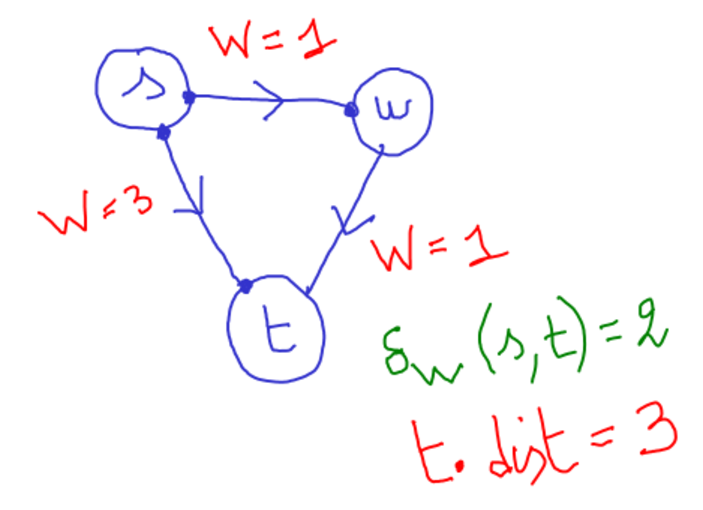
\includegraphics[width = 7cm]{data/weighted_missed.pdf}
\end{center}

If we examine the proof of Proposition \ref{prop:shortest}, the only place where
the adaptation from $\delta$ to $\delta_W$ would fail is at the very last step
when we argued that the values of $.dist$ are naturally ordered in the queue
from front to tail, and that as a consequence the values of $.dist$ are
increasing as a function of their time of dequeue. To remedy to this failure,
the simplest and most effective way, as suggested by Dijkstra in 1959, is to 
replace the queue $Q$ by a heap $H$, with the minimal value of $.dist$ on top.
More precisely, the Dijkstra algorithm starting at vertex $s$ is :

\begin{algorithm}[H]
\caption{Dijkstra from source vertex $s$}
\begin{algorithmic}
\Function{Dijkstra}{$s$}
\State create and empty queue H
\State push $s$ into $H$ with $.dist = 0$ and mark $s$ as discovered
\While{$H$ not empty}
\State pop minimal element $v$ from $H$
	\State mark $v$ as visited
	\ForAll{$w \in Adj(v)$}
	\If{$w$ is not marked discovered}
	\State push $w$ into $H$ with $w.pred = v$ and $w.dist = v.dist + W(v,w)$
	\ElsIf{$w.dist > v.dist + W(v,w)$}
	\State update $w.dist = v.dist + W(v,w)$ and $w.pred = v$ in $H$
	\EndIf
	\EndFor
	\EndWhile
	\EndFunction
\end{algorithmic}
\end{algorithm}

We have 

\begin{proposition}\label{prop:dijkstra}
	A target vertex $t \in V$ gets discovered by $Dijkstra(s)$ if and only if $t \in
	Reach(s)$. Moreover, for such vertices the value $t.dist$ contains the actual
	minimal weighted distance from $s$ to $t$ in $G$, i.e.
	$$
	t.dist = \delta_W(s,t).
	$$
	Besides, one (among) shortest path(s) from $s$ to $t$ is 
	obtained (in reverse order) by recursively taking the .pred 
	attribute of the vertices starting from $t$ and until $s$ is reached.
\end{proposition}
\begin{proof}
As already mentioned the proof is an almost immediate adaptation of the one of
Proposition \ref{prop:shortest}, we repeat it for completeness, except for 
part i) which is really identical and can still be performed by induction on
$\delta(s,t)$ (instead of $\delta_W(s,t)$ which wouldn't fit an induction stricto  
sensu).\\

ii) We next show that $t.dist \geq \delta_W(s,t)$, for all $t \in Reach(s).$
We argue by contradiction and consider that smallest value of $t.dist$ for which 
$t.dist < \delta_W(s,t).$ The vertex $t$ cannot be equal to $s$ because
$s.dist = \delta_W(s,s) = 0.$ Therefore $t$ possesses a valid $u :=
t.pred$ and by construction $t.dist = u.dist + W(u,t).$ Since $W$ is
positive (this is one of the few places where it matters), we have 
$u.dist < t.dist$ and therefore by minimality $u.dist = \delta_W(s,u).$ This in
	turn implies that $\delta_W(s,t) > t.dist = u.dist + W(u,t) =
	\delta_W(s,u) + W(u,t) \geq \delta_W(s,u) + \delta_W(u,t)$, which
	contradicts the triangle inequality for $\delta_W.$ 

iii) We finally show that $t.dist = \delta(s,t)$, for all $t \in Reach(s).$
Assume again by contradiction that this is false, and let $t \in Reach(s)$ be
a vertex for which equality fails, and among these one with the smallest
value (noted $d$) of $\delta_W(s,t).$ By construction and ii), we necessarily  have
$$
d = \delta_W(s,t) < t.dist.
$$
Let $(v_i)_{0 \leq i \leq \ell}$ be a shortest path in $G$ joining $s$
to $t$, and let $v := v_{\ell - 1}.$ By the sub path optimality property 
we have $\delta_W(s,v) = d - W(v_{\ell-1} < d$ and therefore by the minimality
assumption about $d$ we have $\delta_W(s,v) = v.dist.$  At the time $v$ is
marked {\it visited} by BFS(s), we distinguish two cases.\\
Case 1: $t$ is not yet
visited. In that case following BFS(s) we should have set $t.dist =
v.dist + W(v,t)$ (if $t$ was also not discovered) or $t.dist =
\min(t.dist, v.dist + W(v,t))$ (in case $t$ was already discovered). Besides,
the value of $t.dist$ could then only have been lowered later in an
update, and the value of $v.dist$ will no longer change since by assumption $v$
was just visited. Therefore eventually we would still have   
$t.dist \leq v.dist + W(v,t)$. But then 
$t.dist \leq v.dist + W(v,t) = (d- W(v,t)) + W(v,t) = d = \delta_W(s,t)$, 
which contradicts the (by contradiction) assumption.\\
Case 2: $t$ was already visited. That instead would lead to the conclusion
that $t.dist \leq v.dist$ (see hereafter), and therefore $t.dist \leq v.dist =
\delta_W(s,v) = \delta_W(s,t) - W(v,t) \leq \delta_W(s,t)$, which again is a 
contradiction. The fact that $t.dist \leq v.dist$ when $t$ is marked visited 
before $v$ is a consequence of the fact that at each step in BFS(s) the smallest 
$.dist$ value in the heap is extracted (by definition of min heap
extraction), and the values that are (potentially) 
then pushed or updated in the heap are strictly larger than the extracted one, 
because $W$ was assumed positive. 
\end{proof}

We finish by discussing the time complexity of the Dijkstra algorithm. For that
purpose, we assume that the heap $H$ is implemented as a binary complete tree,
as we have seen in the corresponding section. Since $H$ contains, at any time 
during the algorithm, at most $|V|$ elements, the cost of each operation (push,
pop, or update) is at most $O(\log(|V|))$. Also, there are at most  $|V|$ push
and pop operations, and at most $|E|$ update operations. The total time
complexity is therefore $O((|V|+|E|)\log(|V|)).$

%%%%%%%%%%%%%%%%%%%%%%%%%%%%%%%%%%%%%%%%%%%%%%%%%%%%%%%%%%%%%%%%%%%%%%%%%%%%%%%
\subsection{Graph traversal \# 2 : Depth First Search (DFS) (TODO)}
%%%%%%%%%%%%%%%%%%%%%%%%%%%%%%%%%%%%%%%%%%%%%%%%%%%%%%%%%%%%%%%%%%%%%%%%%%%%%%%

%%%%%%%%%%%%%%%%%%%%%%%%%%%%%%%%%%%%%%%%%%%%%%%%%%%%%%%%%%%%%%%%%%%%%%%%%%%%%%%
\subsection{Application to Topological sort (TODO)}
%%%%%%%%%%%%%%%%%%%%%%%%%%%%%%%%%%%%%%%%%%%%%%%%%%%%%%%%%%%%%%%%%%%%%%%%%%%%%%%

%%%%%%%%%%%%%%%%%%%%%%%%%%%%%%%%%%%%%%%%%%%%%%%%%%%%%%%%%%%%%%%%%%%%%%%%%%%%%%%
\subsection{Graph cuts and minimal spanning trees (TODO)}
%%%%%%%%%%%%%%%%%%%%%%%%%%%%%%%%%%%%%%%%%%%%%%%%%%%%%%%%%%%%%%%%%%%%%%%%%%%%%%%





%%%%%%%%%%%%%%%%%%%%%%%%%%%%%%%%%%%%%%%%%%%%%%%%%%%%%%%%%%%%%%%%%%%%%%%%%%%%%%%
%%%%%%%%%%%%%%%%%%%%%%%%%%%%%%%%%%%%%%%%%%%%%%%%%%%%%%%%%%%%%%%%%%%%%%%%%%%%%%%
\pagebreak
\section{Meshes (TODO)}
%%%%%%%%%%%%%%%%%%%%%%%%%%%%%%%%%%%%%%%%%%%%%%%%%%%%%%%%%%%%%%%%%%%%%%%%%%%%%%%
%%%%%%%%%%%%%%%%%%%%%%%%%%%%%%%%%%%%%%%%%%%%%%%%%%%%%%%%%%%%%%%%%%%%%%%%%%%%%%%

%%%%%%%%%%%%%%%%%%%%%%%%%%%%%%%%%%%%%%%%%%%%%%%%%%%%%%%%%%%%%%%%%%%%%%%%%%%%%%%
\subsection{Conforming meshes}
%%%%%%%%%%%%%%%%%%%%%%%%%%%%%%%%%%%%%%%%%%%%%%%%%%%%%%%%%%%%%%%%%%%%%%%%%%%%%%%

%%%%%%%%%%%%%%%%%%%%%%%%%%%%%%%%%%%%%%%%%%%%%%%%%%%%%%%%%%%%%%%%%%%%%%%%%%%%%%%
\subsection{Adjacency tables}
%%%%%%%%%%%%%%%%%%%%%%%%%%%%%%%%%%%%%%%%%%%%%%%%%%%%%%%%%%%%%%%%%%%%%%%%%%%%%%%

%%%%%%%%%%%%%%%%%%%%%%%%%%%%%%%%%%%%%%%%%%%%%%%%%%%%%%%%%%%%%%%%%%%%%%%%%%%%%%%
\subsection{Boundary and geometric invariants}
%%%%%%%%%%%%%%%%%%%%%%%%%%%%%%%%%%%%%%%%%%%%%%%%%%%%%%%%%%%%%%%%%%%%%%%%%%%%%%%

%%%%%%%%%%%%%%%%%%%%%%%%%%%%%%%%%%%%%%%%%%%%%%%%%%%%%%%%%%%%%%%%%%%%%%%%%%%%%%%
%%%%%%%%%%%%%%%%%%%%%%%%%%%%%%%%%%%%%%%%%%%%%%%%%%%%%%%%%%%%%%%%%%%%%%%%%%%%%%%
\pagebreak
\section{Sparse matrices (TODO)}
%%%%%%%%%%%%%%%%%%%%%%%%%%%%%%%%%%%%%%%%%%%%%%%%%%%%%%%%%%%%%%%%%%%%%%%%%%%%%%%
%%%%%%%%%%%%%%%%%%%%%%%%%%%%%%%%%%%%%%%%%%%%%%%%%%%%%%%%%%%%%%%%%%%%%%%%%%%%%%%
\subsection{Representations}
\subsection{Computations}
\subsection{Band width reduction}

%%%%%%%%%%%%%%%%%%%%%%%%%%%%%%%%%%%%%%%%%%%%%%%%%%%%%%%%%%%%%%%%%%%%%%%%%%%%%%%
%%%%%%%%%%%%%%%%%%%%%%%%%%%%%%%%%%%%%%%%%%%%%%%%%%%%%%%%%%%%%%%%%%%%%%%%%%%%%%%
\pagebreak
\section{Spatial data structures (TODO)}
%%%%%%%%%%%%%%%%%%%%%%%%%%%%%%%%%%%%%%%%%%%%%%%%%%%%%%%%%%%%%%%%%%%%%%%%%%%%%%%
%%%%%%%%%%%%%%%%%%%%%%%%%%%%%%%%%%%%%%%%%%%%%%%%%%%%%%%%%%%%%%%%%%%%%%%%%%%%%%%

%%%%%%%%%%%%%%%%%%%%%%%%%%%%%%%%%%%%%%%%%%%%%%%%%%%%%%%%%%%%%%%%%%%%%%%%%%%%%%%
\subsection{Spatial hashing}
%%%%%%%%%%%%%%%%%%%%%%%%%%%%%%%%%%%%%%%%%%%%%%%%%%%%%%%%%%%%%%%%%%%%%%%%%%%%%%%

%%%%%%%%%%%%%%%%%%%%%%%%%%%%%%%%%%%%%%%%%%%%%%%%%%%%%%%%%%%%%%%%%%%%%%%%%%%%%%%
\subsection{K-d trees}
%%%%%%%%%%%%%%%%%%%%%%%%%%%%%%%%%%%%%%%%%%%%%%%%%%%%%%%%%%%%%%%%%%%%%%%%%%%%%%%

%%%%%%%%%%%%%%%%%%%%%%%%%%%%%%%%%%%%%%%%%%%%%%%%%%%%%%%%%%%%%%%%%%%%%%%%%%%%%%%
\subsection{R-trees}
%%%%%%%%%%%%%%%%%%%%%%%%%%%%%%%%%%%%%%%%%%%%%%%%%%%%%%%%%%%%%%%%%%%%%%%%%%%%%%%

\end{document}
